In questo capitolo si entrerà nei dettagli che hanno portato alla realizzazione del backend del progetto CAMUS. Il capitolo inizia con la descrizione delle tecnologie che sono state utilizzate e l'analisi dello schema dell'architettura del sistema. In seguito vengono presentati due descrittori che definiscono il comportamento dell'applicazione nelle diverse situazioni di utilizzo, che sono quello dell'albero di contesto e quello dei servizi. Viene mostrato prima il modello concettuale del database, con una descrizione delle entità e relazioni che lo compongono, e successivamente lo schema logico risultante. Una volta definita la base di dati si passa all'analisi dettagliata dei principali componenti che fanno parte del sistema, con l'ausilio di diagrammi e pseudocodice per una maggiore comprensione. Descritti i componenti viene mostrato come dall'esterno è possibile eseguire le attività che il backend mette a disposizione tramite l'unico endpoint fornito da GraphQL. Per una maggiore chiarezza viene mostrato il flusso che una richiesta percorre nel backend affinché venga evasa, mostrando nel dettaglio le varianti che possono verificarsi. In conclusione viene mostrato come è possibile configurare alcuni parametri del sistema per modificarne il comportamento, attraverso variabili d'ambiente e file di configurazione.

\section{Architettura e tecnologie utilizzate\label{sec:architettura-backend}}

Questa sezione è dedicata alla descrizione delle tecnologie che sono state utilizzate per la realizzazione del backend e delle motivazioni che hanno portato alla loro scelta. In seguito verrà esposto com'è stata strutturata l'architettura del sistema e le sue peculiarità.

La logica del sistema è stata realizzata a partire da Node.js\footnote{Node.js: \url{https://nodejs.org/en/}}, un framework per lo sviluppo di applicazioni web basato sul linguaggio Javascript\footnote{Javascript Documentation: \url{https://developer.mozilla.org/en/docs/Web/JavaScript}}. Node.js è basato sul motore Javascript V8 di Google, realizzato con l'obiettivo principale di garantire ottime performance di esecuzione. Il framework permette la creazione di web server tramite l'ausilio di diversi \emph{moduli} che gestiscono le funzionalità di base, come il file system, le operazioni di rete, la crittografia, ecc. \upe compatibile con i sistemi operativi più diffusi e possono essere utilizzati tutti i linguaggi che una volta compilati producono codice Javascript, come CoffeScript o TypeScript. Per certi versi Node.js può essere considerato molto simile a PHP come ambito di utilizzo, la principale differenza è che le funzioni in Node.js non sono bloccanti, quindi è possibile eseguire attività in parallelo e utilizzare callback o promise per gestire il flusso di esecuzione, sia in caso positivo che negativo. Questa scelta di utilizzare un'architettura di tipo \emph{event-driven} permette la realizzazione di web server estremamente scalabili senza coinvolgere l'utilizzo dei thread. Node.js infatti lavora solo su un singolo core, tranne ne caso in cui vengano avviate più istanze separate. Il parallelismo gestito tramite eventi permette di simulare un sistema multithread, riducendo però in maniera significativa la complessità di sviluppo.

Come database è stato scelto di utilizzare MongoDB\footnote{MongoDB: \url{https://www.mongodb.org/}}. MongoDB fa parte della categoria NoSQL, in quanto abbandona lo schema relazionale classico basato su tabelle in favore di uno basato sui documenti. Ogni documento ha una struttura simile ad un file JSON, che in MongoDB viene nominato BSON. A differenza dei database relazionali che hanno uno schema ben definito a priori, in MongoDB viene preferito uno schema dinamico, cioè che varia in base alle esigenze dello sviluppatore. Questa caratteristica permette di sviluppare in maniera più semplice e rapida le applicazioni e di integrare facilmente determinate tipologie di dato. La struttura a documento prevede però un approccio differente nella fase di modellazione, in quanto applicare uno schema adatto ad un sistema relazionale in MongoDB porterebbe a diverse inefficienze. Per esempio, chi è abituato ad un database relazionale deve essere consapevole che in MongoDB non esiste l'operatore di JOIN, bensì viene fornita la possibilità di salvare dei sotto-documenti all'interno di un documento. Per esempio, se si vuole memorizzare un libro che ha più autori è possibile salvare l'elenco degli autori, insieme ad eventuali altri suoi dati, all'interno del documento contenente le informazioni del libro\footnote{Questo è solo un esempio indicativo, non è una soluzione ottima in quanto un autore può pubblicare più di un libro e utilizzando questo schema si otterrebbe duplicazione delle informazioni}. Un'altra caratteristica di MongoDB è la flessibilità nel comporre le query, che possono essere specificate sui campi, su un range di valori o tramite un'espressione regolare. Sono sempre ammesse proiezioni degli attributi che si vogliono visualizzare nei risultati. Sempre per interrogare i dati si possono utilizzare funzioni \emph{MapReduce} e di \emph{aggregazione}. In particolare quest'ultima permette di ottenere un risultato simile all'operatore GROUP BY dei database SQL, ma fornisce inoltre la flessibilità di concatenare più operazioni per formare una \emph{pipeline}. Mette a disposizione anche il comando \emph{\$lookup} per effettuare un'unione tra documenti diversi, al fine di simulare un'operazione di JOIN. MongoDB permette di definire degli \emph{indici} sui campi che vengono utilizzati di frequente nelle query per velocizzarne l'esecuzione. Una caratteristica che rende MongoDB estremamente scalabile è la possibilità di eseguire multiple istanze su macchine diverse, permettendo al sistema di scalare orizzontalmente. Sarà compito di MongoDB gestire le chiamate e selezionare il nodo dove effettuare la richiesta, tramite un sistema di load-balancing. Questa caratteristica viene agevolata dalla struttura del file system utilizzato da MongoDB, chiamato \emph{Grid File System}, che gestisce la divisione dei documenti in diversi \virgolette{pezzi}. Oltre al load-balancing, che viene utilizzato per migliorare le prestazioni, è possibile anche utilizzare altre macchine come \emph{repliche}, in modo da garantire la sicurezza dei dati nel caso di guasti.

Il fatto che MongoDB memorizzi i file in un formato dalla struttura molto simile ad un JSON agevola l'integrazione con Node.js, che a sua volta utilizza oggetti semplicemente convertibili in formato JSON. Come specificato precedentemente, MongoDB non possiede una struttura definita a priori. Per garantire comunque una consistenza dei dati salvati nel database, si è scelto di forzare l'utilizzo di uno schema ben definito tramite un Object Relational Mapping (ORM)\footnote{Object Relational Mapping: \url{https://it.wikipedia.org/wiki/Object-relational_mapping}}. Un ORM fornisce un livello di astrazione superiore ad un driver nativo e permette di specificare come gli oggetti vengono mappati nel database e viceversa, definendo implicitamente uno schema del database. In particolare, per il progetto CAMUS è stato utilizzato un ORM specifico per Node.js di nome mongoose\footnote{MongooseJS: \url{http://mongoosejs.com/}}.

Oltre ad un database che garantisse la persistenza dei dati più importanti, si è resa necessaria l'adozione di un altro database per effettuare  caching delle risposte ricevute dai servizi e per mantenere memorizzate informazioni relative alle sessioni degli utenti. La scelta in questo caso è ricaduta su Redis\footnote{Redis: \url{http://redis.io/}}. Redis fornisce un database interamente memorizzato in memoria, quindi estremamente rapido nell'evadere le richieste, basato su di una struttura di tipo \emph{chiave-valore}. Queste caratteristiche, insieme al fatto che quanto viene salvato un dato è possibile impostare un intervallo di tempo scaduto il quale l'elemento viene eliminato, lo ha reso il candidato perfetto per svolgere questo compito. Per interfacciare Node.js con l'istanza di Redis in esecuzione viene utilizzato il modulo ioredis\footnote{ioredis: \url{https://github.com/luin/ioredis}}.

Infine, per gestire le funzionalità del server viene utilizzato il web framework ExpressJS\footnote{ExpressJS: \url{http://expressjs.com/}}.

\begin{figure}[ht]
	\centering
	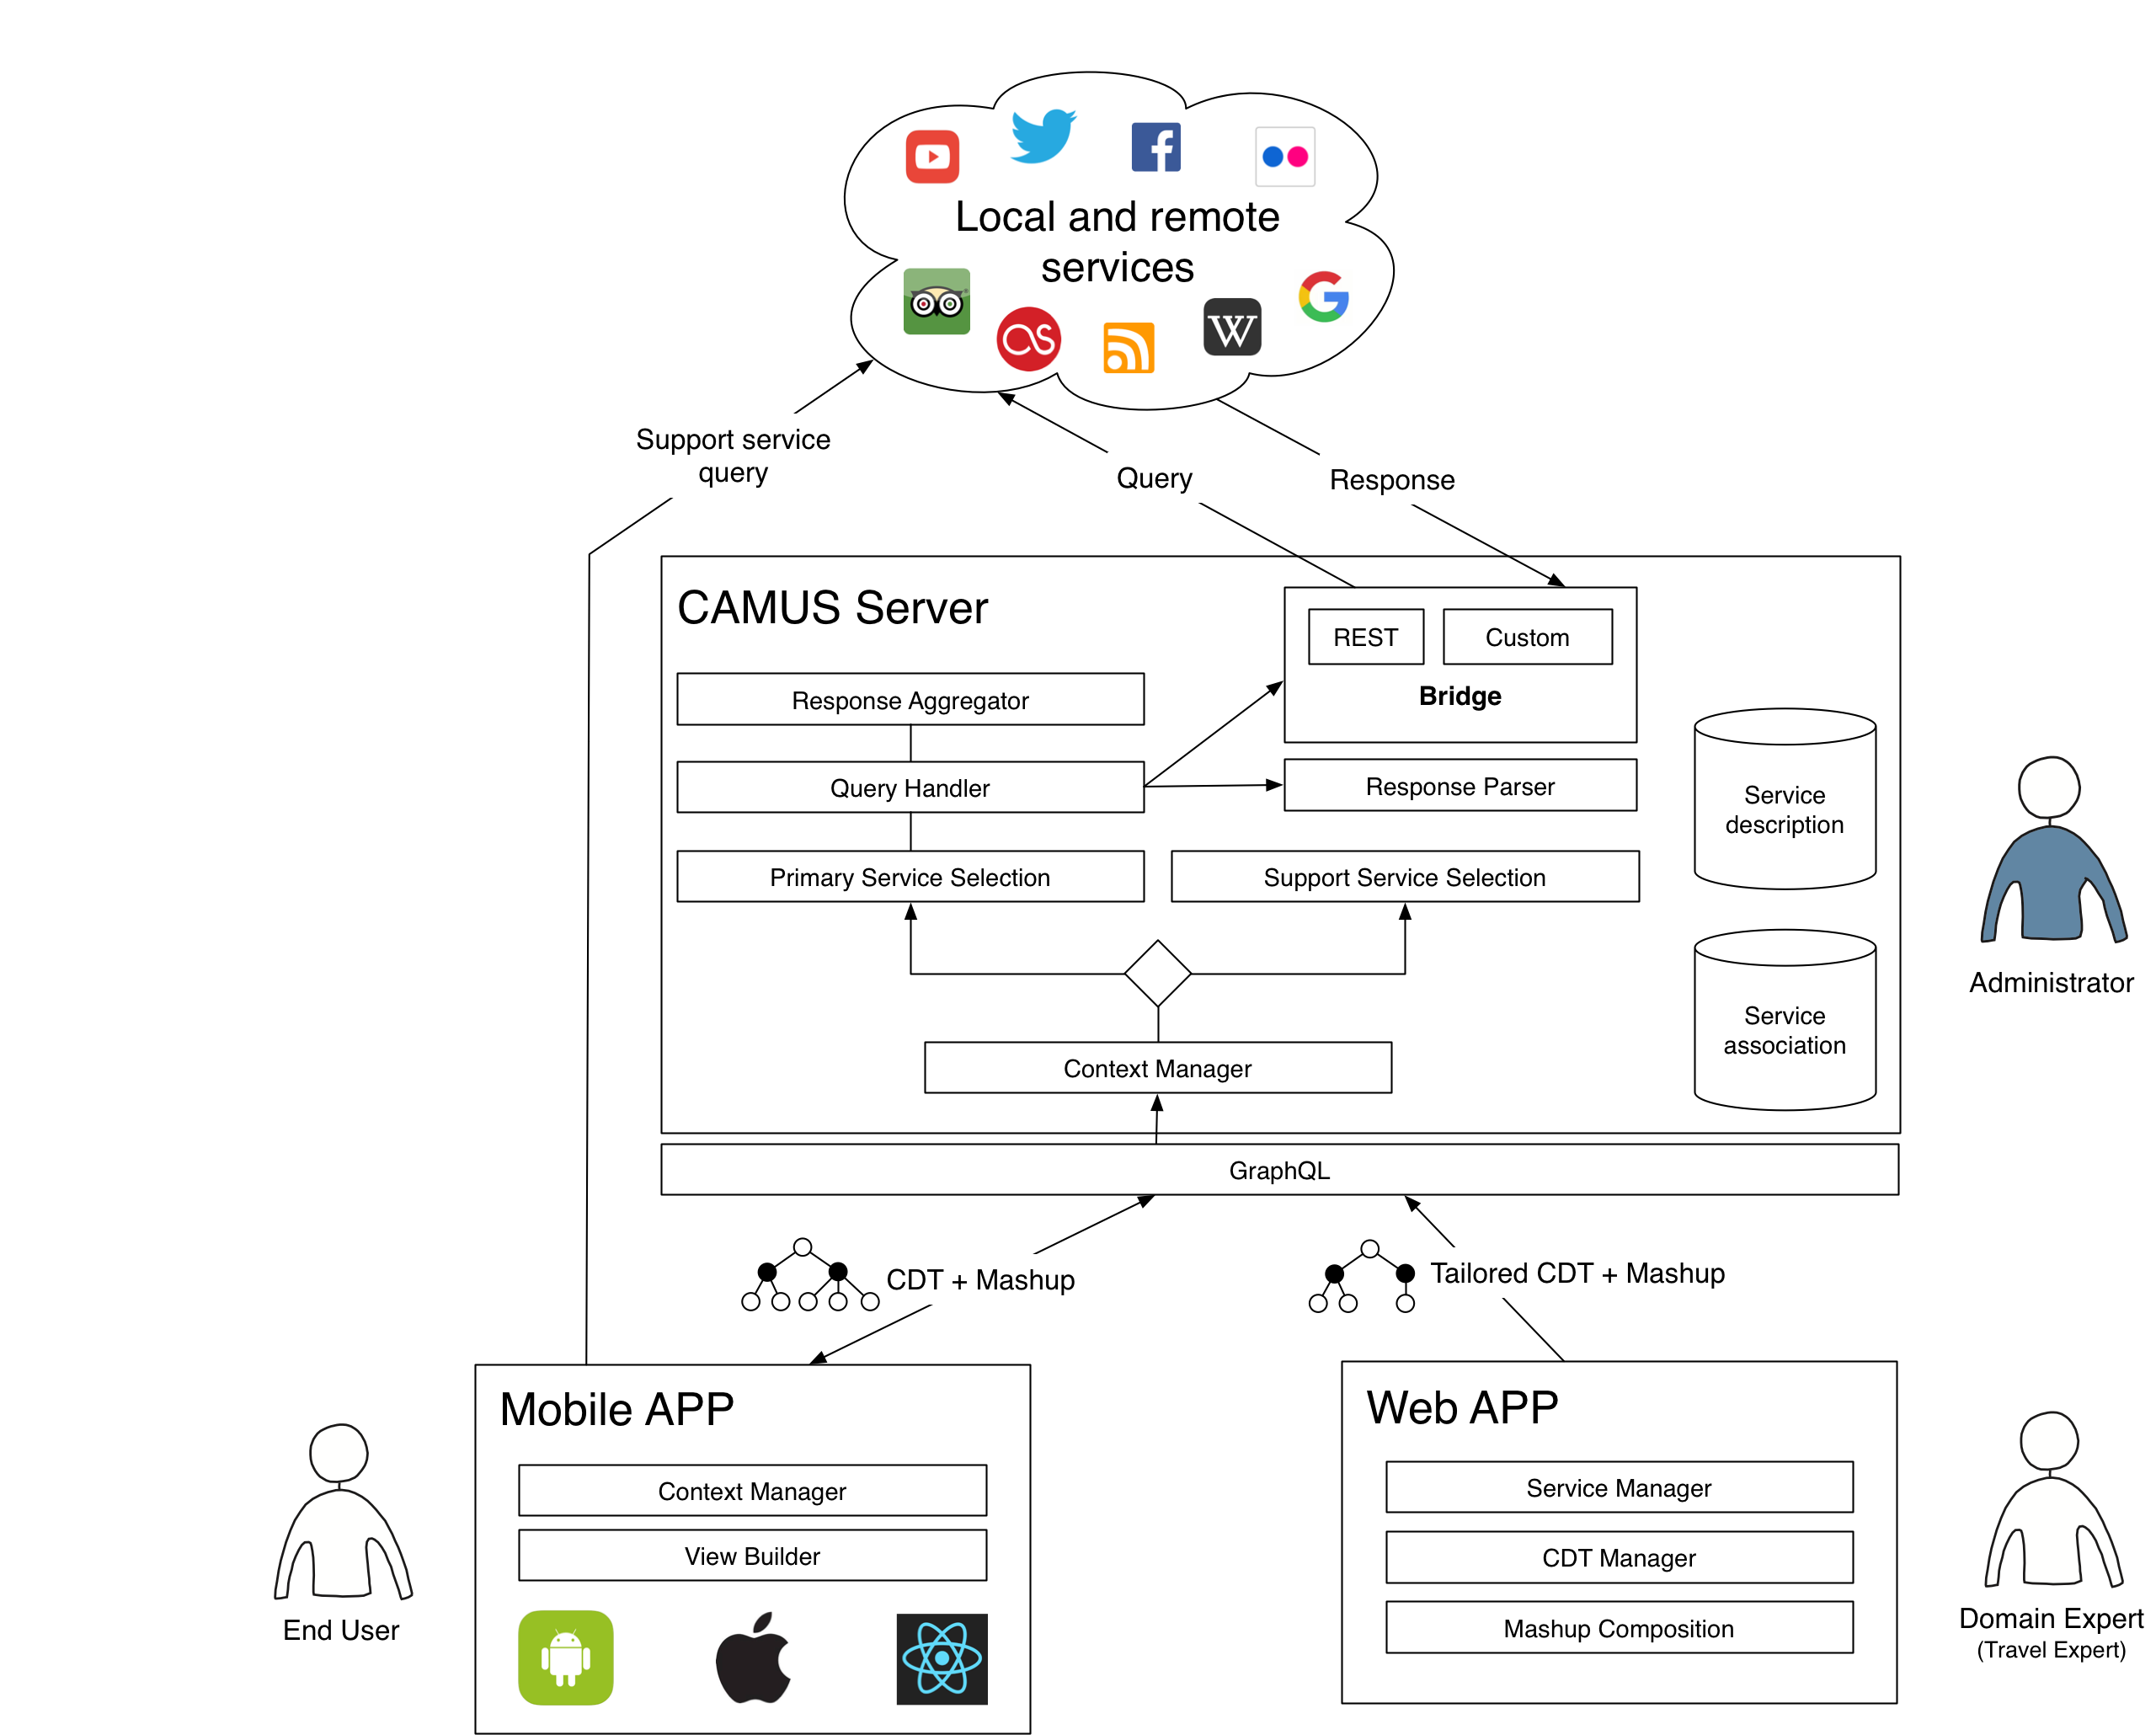
\includegraphics[width=\textwidth]{5-implementazione-backend/Immagini/camus-architecture.png}
	\caption{Architettura del backend}\label{fig:architettura-backend}
\end{figure}

Ora che sono state definite le tecnologie utilizzate viene presentata l'architettura di CAMUS, che può essere osservata nello schema in Figura \ref{fig:architettura-backend}. Come si può notare è stata privilegiata la modularità dei vari componenti che formano il sistema, in modo che ognuno sia circoscritto ad uno specifico compito. Inoltre tutti i componenti mostrati sono \emph{stateless}, cioè non mantengono informazioni sullo stato di una sessione. Questa scelta architetturale permette di poter avviare diverse istanze del backend di CAMUS in modo che le richieste degli utenti possano essere evase da un'istanza piuttosto che un'altra. Questa scelta permette di selezionare quale nodo sia il miglior candidato per gestire una richiesta in coda in base a diverse politiche che non riguardano lo stato della sessione (es.: disponibilità del nodo, basso carico sul sistema, ecc.).

Il componente che coordina tutti gli altri è l'\emph{Execution Helper}. Il suo compito è quello di inizializzare tutti gli altri componenti ed organizzare le chiamate secondo il flusso della richiesta, che verrà analizzato nel dettaglio nella Sezione \ref{sec:flusso-richiesta-server}.

Il \emph{Context Manager} è il componente che si occupa di ricevere il contesto inviato dalla mobile app e lo trasforma in una versione \virgolette{decorata}, eseguendo un'unione tra le informazioni ricevute dal client e quelle del descrittore completo del CDT. In questo modo viene agevolata l'esecuzione dei componenti successivi, in quanto le informazioni necessarie all'elaborazione sono già state catalogate e definite in modo corretto.

Il compito del \emph{Primary Service Selection} è di andare a recuperare le associazioni tra l'albero di contesto e le operazioni dei servizi primari. \upe inoltre suo compito gestire le associazioni personalizzate, come quella relativa la ricerca tramite \emph{località}. In seguito assegna un \emph{punteggio} ad ogni operazione identificata ed emette in uscita le prime N operazioni con valutazione più elevata.

Un compito simile viene svolto dal \emph{Support Service Selection} per le operazioni di supporto. Sebbene lo scopo del componente sia lo stesso, l'algoritmo di selezione è differente: in questo caso le associazioni vengono considerate più come \emph{vincoli}, ed un'operazione, per essere selezionata, deve rispettare tutti i vincoli ad essa associati.

Il \emph{Query Handler} ha il compito di gestire le chiamate verso i servizi. Acquisisce la lista di operazioni scelte dal \emph{Primary Service Selection} e ne recupera i \emph{descrittori}, contenenti le informazioni per poterli interrogare. Di seguito organizza le chiamate ai servizi attraverso l'uso di \emph{bridge} specifici, che sono scelti in base al \emph{protocollo} di comunicazione adottato dal servizio. Una volta ricevute le risposte si occupa di interfacciarsi con il \emph{Response Parser} per trasformarle nella rappresentazione interna, che sfrutta dei \emph{termini semantici} come nome dei campi.

Infine il \emph{Response Aggregator} ha il compito di analizzare gli elementi ricevuti al fine di rimuovere i duplicati.

La gestione di una richiesta che è seguito di una o più effettuate nel passato viene demandata al \emph{Session Helper}. Questo componente si occupa di analizzare lo stato della richiesta e se necessario effettua nuove richieste verso i servizi per acquisire ulteriori informazioni.

Per quanto riguarda l'esposizione dei metodi che possono essere richiamati dal client si è deciso di non utilizzare un approccio basato sull'esposizione di endpoint REST bensì di sperimentare GraphQL, un linguaggio per effettuare interrogazioni creato da Facebook.

GraphQL permette di creare degli \emph{schemi} che definiscono le funzionalità che sono esposte dal sistema e specificano quali dati e in che formato verranno utilizzati sia in ingresso sia in uscita. L'utilizzo di schemi permette di effettuare validazione delle scelte effettuate dal client ed il grosso vantaggio è che sarà GraphQL ad occuparsene, sgravando lo sviluppatore del servizio di questo compito.

Questo discorso viene sempre applicato ai dati in ingresso, in quanto è obbligatorio svolgere una validazione dei dati per ragioni di sicurezza\footnote{\virgolette{Never trust the client}: \url{https://en.wikipedia.org/wiki/Defensive_programming}} ma, come si è notato nel punto precedente, si è parlato anche di informazioni in uscita. Questa è un'altra particolarità di GraphQL, che non è presente negli approcci di tipo REST. Il formato delle risposte non viene deciso dal server bensì è il client a richiedere solamente i dati che gli servono. Questa idea nasce dal fatto che è il client l'utilizzatore finale del servizio ed è la parte del sistema che meglio conosce quali dati gli servono. GraphQL permette di definire schemi anche per le risposte, in modo che i client possano avere una descrizione formale di quali dati possono ricevere.

Per richiamare un endpoint GraphQL viene utilizzato un indirizzo unico esposto da GraphQL. Sarà poi lo schema definito in precedenza a gestire le successive fasi dell'interazione, specificano quale attività specifica si desidera utilizzare.

Assieme alla specifica del linguaggio sono state rilasciate le implementazioni specifiche per la creazione degli schemi in Javascript\footnote{GraphQL-js: \url{https://github.com/graphql/graphql-js}} ed il plug-in per ExpressJS\footnote{Express-GraphQL: \url{https://github.com/graphql/express-graphql}}.

Ulteriori dettagli su GraphQL sono stati mostrati nella Sezione \ref{sec:graphql-introduzione}. 

In questa sezione si è voluta dare una visione d'insieme sui compiti che spettano ai vari componenti. Un'analisi più approfondita delle attività di ognuno di essi verrà svolta nella Sezione \ref{sec:componenti-backend}.

\section{Descrittore dell'albero di contesto\label{sec:descrittore-albero-contesto}}

Nella Sezione \ref{sec:context-dimension-model} è stato esposto il modello teorico del \emph{Context Dimension Tree} mentre in questa sezione si vuole mettere in risalto come l'albero di contesto viene descritto nel sistema. Sono state effettuate diverse semplificazioni per agevolare la memorizzazione ed il recupero delle informazioni dei vari nodi che compongono l'albero. Nelle seguenti sottosezioni vengono analizzati nel dettaglio i singoli oggetti che formano un albero di contesto.

\subsection{Radice\label{sec:radice-cdt}}

Questo oggetto rappresenta la radice di un albero di contesto. \upe composto dai seguenti parametri:

\begin{itemize}
	\item \textbf{User Id} L'elenco degli identificativi degli utenti ai quali questo albero è indirizzato. Viene lasciata la possibilità di definire più utenti perché uno stesso albero può essere valido per più utenti con un profilo simile
	\item \textbf{Context} Contiene i \emph{nodi} che compongono l'albero. Per una descrizione approfondita si fa riferimento alla Sezione \ref{sec:nodo-cdt}
	\item \textbf{Default Values} Vengono elencati tutti i valori che l'\emph{esperto di settore} ha deciso siano sempre validi per gli utenti ai quali questo albero viene associato. \upe composto dal nome della \emph{dimensione} e dal relativo \emph{valore} che assume
\end{itemize}

Viene inoltre definito un \emph{CDT Globale}, utilizzato come base per la creazione di quelli specifici per ogni utente. Questo albero ha la particolarità che non è associato a nessun utente.

\subsection{Nodi\label{sec:nodo-cdt}}

Questo oggetto rappresenta un nodo dell'albero. In particolare vengono rappresentati solamente i nodi di tipo \emph{dimensione} tramite oggetti dedicati, mentre i nodi \emph{contesto} e \emph{parametro} vengono rappresentati come sottocomponenti. Ogni nodo possiede i seguenti attributi:

\begin{itemize}
	\item \textbf{Name} Il nome del nodo dimensione
	\item \textbf{For} Descrive la tipologia di nodo, che verrà utilizzata per assegnare un peso utile nella fase di \emph{selezione delle operazioni} e per attribuire un valore ai parametri nella fase di \emph{invocazione dei servizi}. I valori ammessi sono \emph{filter}, \emph{parameter} o \emph{ranking}. Vengono inoltre ammesse le combinazioni \emph{filter}|\emph{parameter} e \emph{ranking}|\emph{parameter}: un nodo può essere solamente di tipo \emph{filter} o \emph{ranking}, al fine dell'assegnamento dei pesi, mentre può essere anche di tipo \emph{parameter}, in quanto indica che verrà utilizzato anche nella fase di composizione delle query. Se viene definito il tipo \emph{parameter} devono essere assegnati diversi \emph{parametri}, per specificarne le caratteristiche
	\item \textbf{Values} Elenca i possibili valori che può assumere il nodo. Questo elenco corrisponde ai nodi di tipo \emph{contesto} del modello del CDT
	\item \textbf{Parameters} L'elenco dei parametri associati al nodo. Per ulteriori dettagli su questo oggetto si fa riferimento alla Sezione \ref{sec:parametro-cdt}
	\item \textbf{Parents} Contiene l'elenco di tutti i nodi dimensione dai quali discende il nodo corrente. Viene utilizzato per effettuare l'unione delle sottodimensioni di un nodo
\end{itemize}

Nel Listato \ref{lst:esempio-nodo-cdt} viene mostrato un esempio di nodo.

\begin{lstlisting}[style=blocco-esempi,
								caption=Esempio di nodo del CDT,
								label=lst:esempio-nodo-cdt]
	{
		"name": "InterestTopic",
		"for": "filter",
		"values": [
			"Restaurant",
			"Cinema",
			"Theater",
			"Hotel",
			"Museum",
			"Event"
		]
	}
\end{lstlisting}

\subsection{Parametri\label{sec:parametro-cdt}}

Questo oggetto definisce i parametri che sono associati ad un nodo dimensione. Corrisponde ai nodi di tipo \emph{parametro} del modello del CDT. I parametri vengono utilizzati per permettere all'utente di specificare dei valori di sua scelta (es.: località). \upe composto dai seguenti campi:

\begin{itemize}
	\item \textbf{Name} Il nome del parametro, che deve essere lo stesso che l'operazione definisce. Questo campo verrà utilizzato in fase di composizione della query per invocare il servizio ed è quindi essenziale che equivalga al nome fornito dal gestore del servizio
	\item \textbf{Type} Il/I formato/i del dato che vengono accettati
	\item \textbf{Fields} Questo elenco permette di definire dei campi che vanno ulteriormente a specificare il parametro. Un esempio viene dato dal parametro \virgolette{Località}, che può essere specializzato nei campi \virgolette{Latitudine} e \virgolette{Longitudine}
\end{itemize}

Nel Listato \ref{lst:esempio-parametro-cdt} viene mostrato un esempio di parametro.

\begin{lstlisting}[style=blocco-esempi,
								caption=Esempio di parametro associato ad un nodo,
								label=lst:esempio-parametro-cdt]
	{
		"name": "Location",
		"for": "ranking|parameter",
		"parameters": [
			{
				"name": "CityCoord",
				"fields": [
					{
						"name": "Latitude"
					},
					{
						"name": "Longitude"
					}
				]
			}
		]
	}
\end{lstlisting}

\section{Descrittore dei servizi\label{sec:descrittore-servizi}}

In CAMUS l'acquisizione dei dati avviene tramite servizi, come descritto nella Sezione \ref{sec:utilizzo-servizi}. Affinché il sistema possa effettuare le richieste è necessario che sia presente una formato per descrivere le caratteristiche di ogni servizio (es.: l'indirizzo verso il quale effettuare la richiesta, i parametri da inserire, ecc.). Per questo motivo è stato introdotto l'utilizzo di un \emph{descrittore dei servizi}, che sia in grado di descrivere tutte le possibili configurazioni che i servizi possono richiedere. I \emph{descrittori} non sono altro che configurazioni dei servizi espressi tramite file JSON. Di seguito verranno analizzati nel dettaglio tutti i campi che compongono il descrittore. Visto che il descrittore contiene una moltitudine di informazioni che riguardano diversi aspetti di un servizio, viene diviso in sotto-oggetti in modo da semplificarne la comprensione e la lettura.

\subsection{Oggetto principale\label{sec:oggetto-principale-servizi}}

\upe il punto di partenza per la descrizione di un servizio. Comprende i seguenti campi:

\begin{itemize}
	\item \textbf{Name} Il nome del servizio
	\item \textbf{Description} Fornisce una descrizione delle funzionalità del servizio
	\item \textbf{Protocol} Definisce la tipologia con la quale accedere al servizio. Può assumere i valori \virgolette{rest}, \virgolette{query} o \virgolette{custom}, per specificare rispettivamente che il servizio viene invocato secondo la logica REST, viene composta una query con parametri o necessita di un metodo particolare per l'accesso
	\item \textbf{Base Path} Rappresenta l'indirizzo di base del servizio. A partire da questo indirizzo verrà composto quello completo aggiungendo in coda i percorsi specifici delle \emph{operazioni} richieste. Non deve essere inserita al termine nessuna slash (\virgolette{/})
	\item \textbf{Operazioni} L'elenco delle operazioni esposte dal servizio. Per un approfondimento riguardo questo oggetto fare riferimento alla Sezione \ref{sec:descrittore-operazioni}
\end{itemize}

Nel Listato \ref{lst:esempio-descrittore-servizio} viene mostrato un esempio di oggetto principale del servizio.

\begin{lstlisting}[style=blocco-esempi,
								caption=Esempio di servizio,
								label=lst:esempio-descrittore-servizio]
  {
	  "name": "GooglePlaces",
	  "protocol": "query",
	  "basePath": "https://maps.googleapis.com/maps/api/place",
	  "operations": [ ... ]
  }
\end{lstlisting}

\subsection{Operazioni\label{sec:descrittore-operazioni}}

Rappresenta le operazioni che sono messe a disposizione dal servizio. Un'operazione viene descritta dai seguenti campi:

\begin{itemize}
	\item \textbf{Name} Il nome dell'operazione
	\item \textbf{Type} Rappresenta la tipologia dell'operazione. Un'operazione può essere \emph{primaria} o di \emph{supporto}. Questa distinzione viene utilizzata principalmente per permettere la catalogazione delle operazioni da mostrare nelle web app
	\item \textbf{Description} La descrizione dell'attività svolta dall'operazione
	\item \textbf{Path} Il percorso specifico per richiamare l'operazione. Questo valore viene aggiunto al \emph{Base Path} del servizio. Deve essere sempre preceduto da una slash (\virgolette{/})
	\item \textbf{Bridge Name} Questo campo è opzionale, definisce il nome del bridge con la logica necessaria per invocare il servizio. \upe obbligatorio il suo utilizzo quando per il servizio viene utilizzato il protocollo \emph{custom}
	\item \textbf{Parameters} Definisce l'elenco dei parametri accettati in ingresso dall'operazione. Per ulteriori dettagli su questo oggetto si fa riferimento alla Sezione \ref{sec:descrittore-parametri}
	\item \textbf{Headers} Permette di specificare gli attributi da aggiungere all'header della richiesta. Vengono utilizzati i campi \virgolette{name} per specificare il nome dell'attributo e \virgolette{value} per specificarne il valore
	\item \textbf{Response Mapping} Serve per definire le regole di associazione per mappare la risposta del servizio coi termini semantici utilizzati dal sistema. Maggiori dettagli su questo oggetto vengono discussi nella Sezione \ref{sec:descrittore-risposta}
	\item \textbf{Pagination} Serve a raccogliere gli attributi necessari per gestire la paginazione specifica di ogni servizio. Sono supportati meccanismi di paginazioni basati sul \emph{numero di pagina} o su \emph{token}. Questo oggetto viene analizzato nel dettaglio nella Sezione \ref{sec:descrittore-paginazione}
\end{itemize}

Nel Listato \ref{lst:esempio-descrittore-operazione} viene mostrato un esempio di operazione.

\begin{lstlisting}[style=blocco-esempi,
								caption=Esempio di operazione,
								label=lst:esempio-descrittore-operazione]
	{
		"name": "nearBySearch",
		"type": "primary",
		"path": "/nearbysearch/json",
		"parameters": [ ... ],
		"responseMapping": { ... },
		"pagination": { ... }
	}
\end{lstlisting}

\subsection{Parametri\label{sec:descrittore-parametri}}

In quest'oggetto vengono definiti i parametri in ingresso di un'operazione. I parametri generalmente sono composti da un campo che ne definisce il \emph{nome} e dal rispettivo \emph{valore}. In alcuni casi però vengono accettati più di un valore. Il descrittore deve dunque essere in grado di gestire questa situazione. Un ulteriore compito affidato a questo oggetto è quello di acquisire il valore di un determinato parametro dal \emph{contesto}. Viene inoltre fornito un semplice sistema di traduzione dei dati acquisiti dal contesto, per permettere le trasformazioni verso un valore idoneo per l'operazione corrente. Infine, soprattutto per le operazioni di \emph{supporto}, viene permessa un'associazione del parametro verso uno o più \emph{termini semantici}, per permettere all'app mobile di conoscere l'attributo dove andare a recuperare il valore concreto a run-time. Nello specifico, l'oggetto è così composto:

\begin{itemize}
	\item \textbf{Name} Il nome del parametro. Questo campo è \emph{obbligatorio}, in quanto definisce il nome che verrà utilizzato per comporre la query per richiedere i dati
	\item \textbf{Description} La descrizione della tipologia del parametro
	\item \textbf{Required} Specifica se il parametro corrente è obbligatorio o meno in una richiesta. Non definire questo attributo equivale ad assegnargli valore \emph{false}
	\item \textbf{Type} Definisce il \emph{tipo} di dato che l'operazione si aspetta di ricevere. Le principali tipologie di dato che vengono inviate verso i servizi sono \emph{stringhe}, \emph{numeri} o \emph{date}
	\item \textbf{Default} Indica un valore predefinito per il parametro. Questo campo è particolarmente utile per la web app relativa il \emph{Visual Mapping}, in quanto permette di ricevere degli esempi di risposta dei servizi da mostrare all'utente
	\item \textbf{Collection Format} Questo campo definisce il \emph{separatore} da utilizzare nel caso siano presenti più di un valore per il parametro. Sono accettati i seguenti quattro separatori: \emph{i)} csv, comma separated values; \emph{ii)} ssv, space separated values; \emph{iii)} tsv, tab separated values; \emph{iv)} pipes. Se non specificato viene utilizzato di default il tipo \emph{csv}
	\item \textbf{Mapping CDT} Definisce uno o più nodi dell'albero di contesto dove andare ad acquisire il valore ricevuto dalla mobile app. Nel caso vengano associati più di un nodo viene seguito l'ordine di definizione nella fase di composizione della query
	\item \textbf{Mapping Term} Definisce uno o più termini semantici da associare al parametro. Questi termini vengono utilizzati a run-time per andare ad acquisire il valore del parametro dalle risposte ricevute dai servizi primari
	\item \textbf{Translate} Permette delle semplici trasformazioni dei valori acquisiti dall'albero di contesto per renderli conformi a quelli accettati dal servizio. \upe formato dai campi \virgolette{from} e \virgolette{to}, che specificano rispettivamente il valore di \emph{origine} e quello \emph{tradotto}. Vengono definite tante traduzioni quanti sono i valori che può assumere il rispettivo nodo del CDT
\end{itemize}

Nel Listato \ref{lst:esempio-descrittore-parametro} viene mostrato un esempio di parametro.

\begin{lstlisting}[style=blocco-esempi,
								caption=Esempio di parametro,
								label=lst:esempio-descrittore-parametro]
	{
		"name": "Location",
		"required": true,
		"default": "-33.8670522,151.1957362",
		"collectionFormat": "csv",
		"mappingCdt": [
			"CityCoord.Latitude",
			"CityCoord.Longitude"
		]
	}
\end{lstlisting}

\subsection{Formato della risposta\label{sec:descrittore-risposta}}

In quest'oggetto sono definite le regole con le quali vengono trasformate le risposte ricevute dal servizio nel formato interno CAMUS, dove ogni attributo viene associato ad un rispetto \emph{termine semantico} che ne definisce il contenuto. In particolare, vengono utilizzati i seguenti campi:

\begin{itemize}
	\item \textbf{List} Definisce l'attributo che contiene l'elenco dei risultati. \upe utile nei casi in cui la risposta, oltre ai risultati, contiene al suo interno anche dei metadati relativi l'interrogazione. Se non specificato si assume che l'elenco dei risultati si trovi nella radice della risposta
	\item \textbf{Items} Permette di mappare i vari campi che compongono ogni oggetto dei risultati. In particolare vengono definiti il \virgolette{percorso} dal quale recuperare il valore ed il \virgolette{termine semantico} da associare. I campi senza un'associazione saranno ignorati dal processo di trasformazione e le relative informazioni andranno perdute. \upe necessario dunque effettuare l'operazione di mapping delle risposte con attenzione, in modo da non trascurare informazioni importanti
	\item \textbf{Functions} Viene permesso l'utilizzo di funzioni specifiche per trasformare i valori. Questa funzione riceve in ingresso il parametro \virgolette{value}, che rappresenta il valore corrente del campo, e deve restituire il nuovo valore che verrà sostituito a quello originale. Oltre alla funzione specifica è necessario definire anche l'\emph{attributo} sul quale eseguire questa trasformazione. L'attributo equivale al \emph{termine semantico} definito nel punto precedente
\end{itemize}

Nel Listato \ref{lst:esempio-formato-risposta} viene mostrato un esempio di formato di risposta.

\begin{lstlisting}[style=blocco-esempi,
								caption=Esempio di formato di risposta,
								label=lst:esempio-formato-risposta]
	{
		"list": "results",
		"items": [
			{
				"termName": "title2,
				"path": "name"
			},
			{
				"termName": "address",
				"path": "vicinity"
			},
			{
				"termName": "latitude",
				"path": "geometry.location.lat"
			},
			{
				"termName": "longitude",
				"path": "geometry.location.lng"
			}
		],
		"functions": [
			{
				"onAttribute": "latitude",
				"run": "return String(value)"
			},
			{
				"onAttribute": "longitude",
				"run": "return String(value)"
			}
		]
	}
\end{lstlisting}

\subsection{Paginazione\label{sec:descrittore-paginazione}}

In quest'oggetto vengono descritti gli attributi necessari per gestire la paginazione delle risposte. In particolare il sistema è in grado di gestire due tecniche di paginazione, quella basata sul \emph{numero di pagina} e quella che utilizza dei \emph{token} per richiamare le pagine. L'oggetto è composto dai seguenti campi:

\begin{itemize}
	\item \textbf{Attribute Name} Specifica il nome del parametro da aggiungere alla query per richiamare una specifica pagina
	\item \textbf{Type} Definisce il meccanismo di paginazione da utilizzare. Sono ammessi due valori: \virgolette{number}, per la paginazione basata sul numero di pagine, e \virgolette{token}, per quella che sfrutta i token per richiamare le pagine successive
	\item \textbf{Token Attribute} Serve per definire dove andare a leggere nella risposta il token relativo alla pagina successiva
	\item \textbf{Page Count Attribute} Definisce l'attributo che fornisce l'informazione del numero di pagine totale che possono essere richieste
\end{itemize}

Nel Listato \ref{lst:esempio-descrittore-paginazione} viene mostrato un esempio di descrittore della paginazione.

\begin{lstlisting}[style=blocco-esempi,
								caption=Esempio di descrittore della paginazione,
								label=lst:esempio-descrittore-paginazione]
	{
		"pagination": {
			"attributeName": "pagetoken",
			"type": "token",
			"tokenAttribute": "next_page_token"
		}
	}
\end{lstlisting}

\section{Schema del database\label{sec:schema-database}}

La base di dati viene utilizzata principalmente per garantire la persistenza di tre elementi: \emph{i)} il descrittore dei servizi, \emph{ii)} l'albero del contesto e \emph{iii)} le associazioni tra operazioni e nodi del CDT.

Queste entità permettono al sistema di svolgere le attività principali. In Figura \ref{fig:schema-er-db} viene mostrato il modello \emph{Entità-Relazione} che sta alla base di CAMUS.

\begin{figure}[ht]
	\centering
	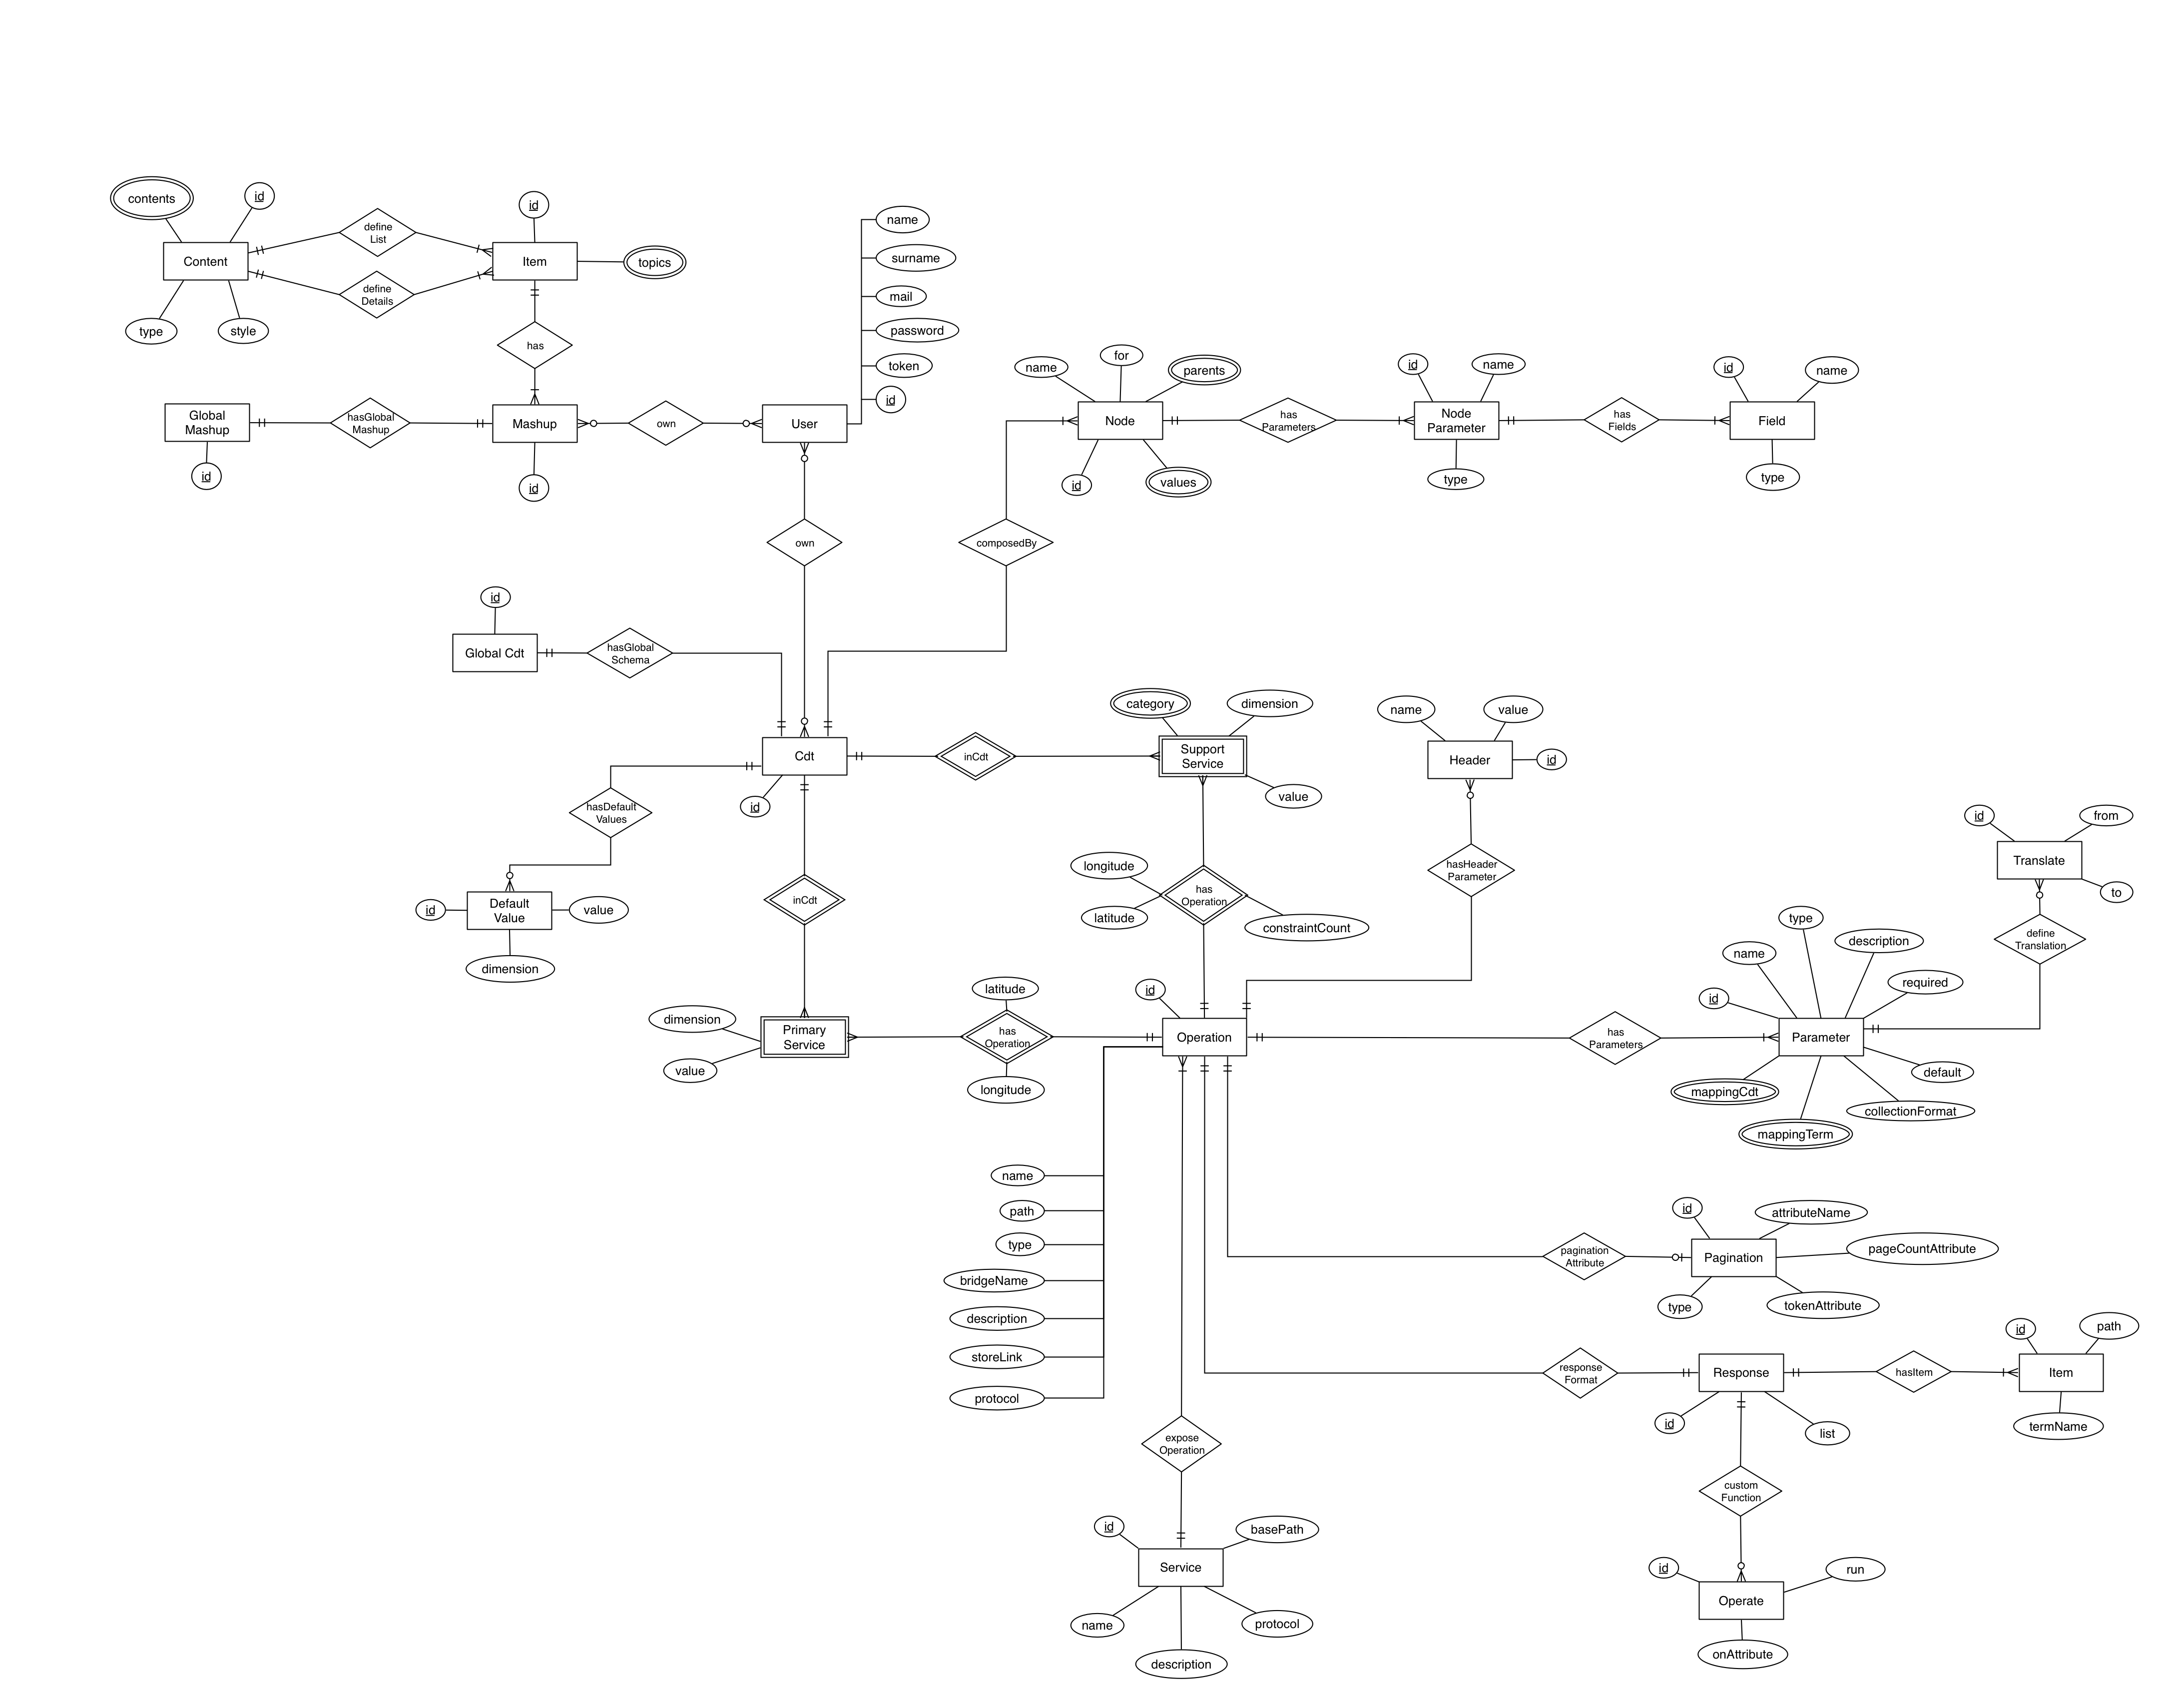
\includegraphics[width=\textwidth]{5-implementazione-backend/Immagini/schema_er_db.png}
	\caption{Diagramma ER del database}\label{fig:schema-er-db}
\end{figure}

Di seguito viene presentata una descrizione dettagliata delle entità che compongono il modello:

\begin{itemize}
	\item \textbf{User} \upe l'entità che rappresenta un utente. Ogni utente viene descritto dal nome, cognome, indirizzo email, password e da un token che viene utilizzato per identificare la sessione. Un utente può possedere nessuno o più CDT
	\item \textbf{Cdt} Rappresenta la radice di un albero di contesto. Un albero di contesto può essere posseduto da zero o più utenti. Il \emph{CDT Globale} è l'unico caso nel quale non vengono associati utenti, perché è universale e quindi valido per chiunque. In tutti gli altri casi si tratta di \emph{CDT su misura}, che devono quindi essere associati ad almeno un utente. Viene lasciata la possibilità di associazione con più utenti nel caso il loro profilo sia molto simile
	\item \textbf{Node} Rappresenta un nodo \emph{dimensione} del CDT e viene descritto dai seguenti attributi:
	\begin{itemize}
		\item \emph{Name} Il nome del nodo
		\item \emph{For} Descrive la tipologia del nodo, che verrà utilizzata per assegnare un peso utile nella fase di \emph{selezione delle operazioni} e per attribuire un valore ai parametri nella fase di \emph{invocazione dei servizi}. I valori ammessi sono \emph{filter}, \emph{parameter}, \emph{ranking}, \emph{filter}|\emph{parameter} o \emph{ranking}|\emph{parameter}. Se viene definito il tipo \emph{parameter} possono essere assegnati al nodo diverse entità di tipo \virgolette{Node Parameter}, per specificarne le caratteristiche
		\item \emph{Parents} Contiene l'elenco di tutti i nodi dai quali discende il nodo corrente
		\item \emph{Values} Elenca i valori ammessi dal nodo dimensione corrente. Corrispondono ai nodi di tipo \emph{contesto} nel modello del CDT
	\end{itemize}
	\item \textbf{Node Parameter} Questa entità rappresenta un parametro associato ad un nodo del CDT. Viene caratterizzato dai seguenti campi:
	\begin{itemize}
		\item \emph{Name} Definisce il nome del parametro
		\item \emph{Type} Il/I formato/i del dato che vengono accettati
	\end{itemize}
	Ad un parametro possono essere associati diversi \virgolette{campi}, nel caso in cui un parametro sia definito da diversi sottoattributi. Per esempio, il parametro \emph{Località} può essere specializzato nei campi \emph{Latitudine} e \emph{Longitudine}
	\item \textbf{Field} \upe l'entità che rappresenta un campo di un parametro. \upe composto dal \virgolette{nome} che assume ed il \virgolette{tipo}, che descrive il formato del campo
	\item \textbf{Default Value} Questa entità elenca le coppie dimensione-valore che sono preimpostate, in quanto non subiscono variazioni per l'utente ed è inutile che gli vengano continuamente riproposte. Vengono salvati solamente il nome della \virgolette{dimensione} ed il relativo \virgolette{valore}
	\item \textbf{GlobalCdt} Entità che mantiene il riferimento al \emph{CDT Globale}, che viene utilizzato come base per la costruzione di tutti gli alberi di contesto del sistema
	\item \textbf{Service} Entità che rappresenta un servizio, definito dai seguenti campi:
	\begin{itemize}
		\item \emph{Name} Il nome del servizio
		\item \emph{Description} Una descrizione delle operazioni che vengono svolte dal servizio
		\item \emph{Base Path} Definisce l'indirizzo base al quale è possibile contattare il servizio. Viene utilizzato insieme ai \emph{path} specifici di ogni operazione per formare l'indirizzo completo
		\item \emph{Protocol} Specifica la tipologia di servizio e può assumere i valori \emph{rest}, \emph{query} o \emph{custom}. Per i primi due casi esiste un'implementazione fornita assieme al sistema mentre per l'ultimo caso è necessario specificare quale bridge specifico viene utilizzato per invocare il servizio
	\end{itemize}
	Un servizio deve esporre almeno un'\emph{operazione} per poter essere utilizzato
	\item \textbf{Operation} Un'operazione rappresenta l'elemento essenziale affinché un servizio possa essere invocato. Possiede i seguenti attributi:
	\begin{itemize}
		\item \emph{Name} Il nome dell'operazione. Questo campo viene utilizzato principalmente per avere un riferimento intuitivo delle varie operazioni che vengono esposte da ogni servizio e può essere scelto a proprio piacimento
		\item \emph{Description} Descrizione dell'attività che viene svolta dall'operazione
		\item \emph{Path} Definisce il percorso specifico verso il quale richiamare l'operazione. Questo campo viene concatenato assieme al \emph{basePath} definito dal servizio per formare l'indirizzo completo
		\item \emph{Type} Specifica se l'operazione è di tipo \emph{primario} o di \emph{supporto}. Questa distinzione è più di carattere categorico che funzionale, in quanto non ci sono particolari variazioni tra le due tipologie di operazione. Viene utilizzato dallo strumento di \emph{Visual Mapping} per elencare nello spazio più appropriato le varie operazioni
		\item \emph{Bridge Name} Questo campo definisce il nome dell'implementazione specifica del bridge da utilizzare per invocare il servizio. \upe necessario solamente nel caso in cui il servizio utilizzi un protocollo \emph{custom}
	\end{itemize}
	Ogni operazione ha una serie di informazioni di contorno che possono essere associate. Deve obbligatoriamente definire un'entità per descrivere il formato della \emph{risposta} che riceve e può esporre gli attributi necessari per gestire la \emph{paginazione} dei risultati. Possono essere associati più campi relativi ai valori da aggiungere all'\emph{header} della chiamata quando necessari. Affinché un'operazione sia utilizzabile, è necessario definire almeno un \emph{parametro} per assegnare i valori che il servizio utilizzerà per comporre la risposta
	\item \textbf{Parameter} Questa entità specifica come sono formati gli attributi che compongono un parametro. In particolare viene descritta dai seguenti campi:
	\begin{itemize}
		\item \emph{Name} Il nome del parametro
		\item \emph{Type} Il formato del valore associato al parametro
		\item \emph{Description} La descrizione della semantica del parametro
		\item \emph{Required} Valore booleano che specifica se il parametro è obbligatorio o meno per l'operazione associata. Di default assume valore \emph{false}
		\item \emph{Default} Specifica un valore predefinito, che viene utilizzato in particolare nella fase di \emph{Visual Mapping} per mostrare una risposta di esempio
		\item \emph{Collection Format} Viene utilizzato solamente nel caso in cui ci siano più valori associati e definisce il separatore da usare per dividere i valori. I separatori riconosciuti sono \emph{csv} (comma separated values), \emph{ssv} (space separated values), \emph{tsv} (tab separated values) e \emph{pipes}.
		\item \emph{Mapping Term} Viene utilizzato per associare il parametro ad uno dei \emph{termini semantici} conosciuti dal sistema. Viene utilizzato per la composizione della query per i servizi di supporto ed accetta la definizione di più termini
		\item \emph{Mapping Cdt} Specifica da quale nodo dell'\emph{albero di contesto} è possibile recuperare il valore da associare al parametro. Possono essere aggiunti più nodi verso i quali andare a cercare i valori
	\end{itemize}
	In alcuni casi può essere anche definita una \emph{traduzione} per permettere di trasformare il valore definito dal contesto in uno più idoneo per il servizio
	\item \textbf{Translate} Questa entità definisce come effettuare una traduzione da un valore, generalmente recuperato dall'albero di contesto, verso un altro riconosciuto dal servizio. Viene semplicemente descritta dai campi \virgolette{from} e \virgolette{to}, che rappresentano rispettivamente il valore originale e la sua traduzione finale
	\item \textbf{Pagination} Specifica quali sono gli attributi della risposta usati per gestire la paginazione dei risultati. In particolare, sono necessarie le seguenti informazioni:
	\begin{itemize}
		\item \emph{Attribute Name} Definisce il nome del parametro utilizzato dall'operazione per richiamare la pagina successiva. Deve corrispondere al nome fornito dal gestore del servizio
		\item \emph{Type} Specifica il tipo di paginazione utilizzata dal servizio. Il sistema supporta due tipologie: \emph{i)} number, dove viene utilizzato un numero per identificare ogni pagina; \emph{ii)} token, dove vengono generati diversi token per richiamare le diverse pagine
		\item \emph{Page Count Attribute} Indica il nome del campo della risposta che contiene il numero totale di pagine che sono disponibili per la query corrente. Viene utilizzato unicamente nel caso sia stato scelto come tipo \emph{number}. Serve al sistema per sapere fino a quando è possibile incrementare il numero di pagina per recuperare nuove informazioni
		\item \emph{Token Attribute} Indica il nome del campo della risposta che contiene il token alla pagina successiva. Viene utilizzato unicamente nel caso sia stato scelto come tipo \emph{token}. Il token recuperato viene utilizzato nella query successiva per richiedere la nuova pagina con altre informazioni. A differenza del caso precedente non è possibile sapere a priori quante siano le pagine in totale. Semplicemente, quando il servizio non fornisce più token significa che non sono più disponibili ulteriori pagine
	\end{itemize}
	\item \textbf{Header} Questa entità definisce gli attributi che devono essere aggiunti all'header di un richiesta. \upe formato dal \virgolette{nome} del campo ed il \virgolette{valore} da associargli
	\item \textbf{Response} \upe l'entità che descrive il formato della risposta ricevuta e definisce come mappare gli attributi che la compongono con i termini semantici. Viene utilizzato il campo \virgolette{list} per specificare il percorso all'interno della risposta dove è possibile andare a recuperare l'elenco dei risultati. Se non specificato viene presa la radice dell'oggetto ricevuto. Inoltre vengono definite diverse associazioni con l'entità \emph{Item}, che definisce come mappare ogni singolo elemento della risposta ai rispettivi termini semantici. In aggiunta è possibile definire delle funzioni che vengono eseguite in seguito alla fase di trasformazione, per permettere la personalizzazione dei valori ricevuti
	\item \textbf{Item} Permette di definire la regola con la quale convertire un campo della risposta nel relativo termine semantico. \upe composto dal campo \virgolette{path}, che specifica il percorso del campo, e \virgolette{termName}, che definisce il termine da associargli
	\item \textbf{Operate} Questa entità permette la creazione di funzioni personalizzate per essere eseguite sui valori ricevuti dal servizio. \upe composta dai campi \virgolette{run}, dove viene scritto il codice (JavaScript) da essere eseguito, e \virgolette{onAttribute}, che specifica il termine coinvolto nella trasformazione. Per l'esecuzione della funzione si tenga presente che viene chiamata fornendo in ingresso il parametro \emph{value}, che corrisponde al valore corrente del campo
	\item \textbf{Primary Service} In questa entità vengono definite le associazioni tra le operazioni primarie e il corrispondente albero del contesto. Viene rappresentata come un'entità debole, in quanto l'identificazione è possibile tramite l'identificativo del CDT e dell'operazione. Non è presente invece una relazione che colleghi quest'entità a quella dei nodi per due motivi in particolare: \emph{i)} per come è stato scelto di rappresentare un nodo non è possibile identificare univocamente una coppia dimensione-valore e \emph{ii)} per ragioni di performance è stato preferito un approccio che richiedesse il coinvolgimento di meno entità possibili. Quindi è stata effettuata una denormalizzazione a livello di modello tramite i campi \virgolette{dimension} e \virgolette{value} che definiscono lo specifico nodo. Viene inoltre permesso di associare un'operazione a delle coordinate geografiche, tramite la relazione \emph{hasOperation}
	\item \textbf{Support Service} In questa entità vengono definite le associazioni tra le operazioni di supporto e il corrispondente albero di contesto. Come per le operazioni primarie, viene anch'essa rappresentata come un'entità debole, in quanto per l'identificazione vengono utilizzati l'identificativo del CDT, quello dell'operazione e la categoria del servizio. Viene seguita la stessa logica di associazione ai nodi utilizzata in precedenza per le operazioni primarie. L'unica variante riguarda l'attributo \virgolette{constraintCount} definito nella relazione \emph{hasOperation}. Come evidenziato nella Sezione \ref{sec:associazione-servizi-cdt}, le associazioni delle operazioni di supporto vengono considerate alla stregua di vincoli, in quanto devono essere tutte rispettate affinché un'operazione possa essere presa in considerazione. Questo attributo viene utilizzato proprio per questo scopo: permette di sapere quanti siano i vincoli definiti per l'operazione corrente e viene utilizzato dell'algoritmo di selezione
	\item \textbf{Mashup} Rappresenta gli schemi dei mashup. Uno schema è composto da uno o più \emph{Item}, che definiscono le regole per la visualizzazione dei risultati. Uno schema può essere associato a diversi utenti, quando condividono un profilo simile. Uno schema può anche non essere associato ad alcun utente: in questo caso si parla si \emph{Mashup Globale}, cioè uno schema che è valido per qualsiasi utente
	\item \textbf{Item} Definisce per quali \emph{topics} lo schema è valido. Le regole di visualizzazione si dividono in due aree: \emph{List}, per gestire l'elenco dei risultati, e \emph{Details}, che rappresenta la pagina di dettaglio di un elemento. Vengono entrambi rappresentati dall'entità \emph{Content}, che ne specifica i dettagli
	\item \textbf{Content} Specifica le regole per visualizzare gli elementi all'interno della schermata specifica. Il campo \emph{type} definisce la tipologia del componente da utilizzare (es.: text, map, ecc.), \emph{style} permette di utilizzare uno stile personalizzato ed infine \emph{contents} che definisce i termini semantici dai quali acquisire le informazioni da mostrare
	\item \textbf{Global Mashup} Questa entità viene utilizzata per acquisire lo schema di \emph{Mashup Globale} nel caso in cui ad un utente non è stato creato uno schema specifico
\end{itemize}

Una volta definito il modello ER è necessario passare alla realizzazione dello \emph{schema logico} del database, quello che verrà effettivamente utilizzato nell'implementazione. Non esistendo uno standard per realizzare uno schema di questo tipo per i database non relazionali è stato scelto di utilizzare un \emph{diagramma delle classi} per rappresentare i \emph{documenti} che compongono il database. Ogni classe viene intesa come un documento ed i collegamenti evidenziati con una linea continua rappresentano i sottodocumenti. Le linee tratteggiate indicano le referenze tra i vari documenti.

In Figura \ref{fig:schema-logico-db} viene mostrato lo schema logico utilizzato per CAMUS.

\begin{figure}[ht]
	\centering
	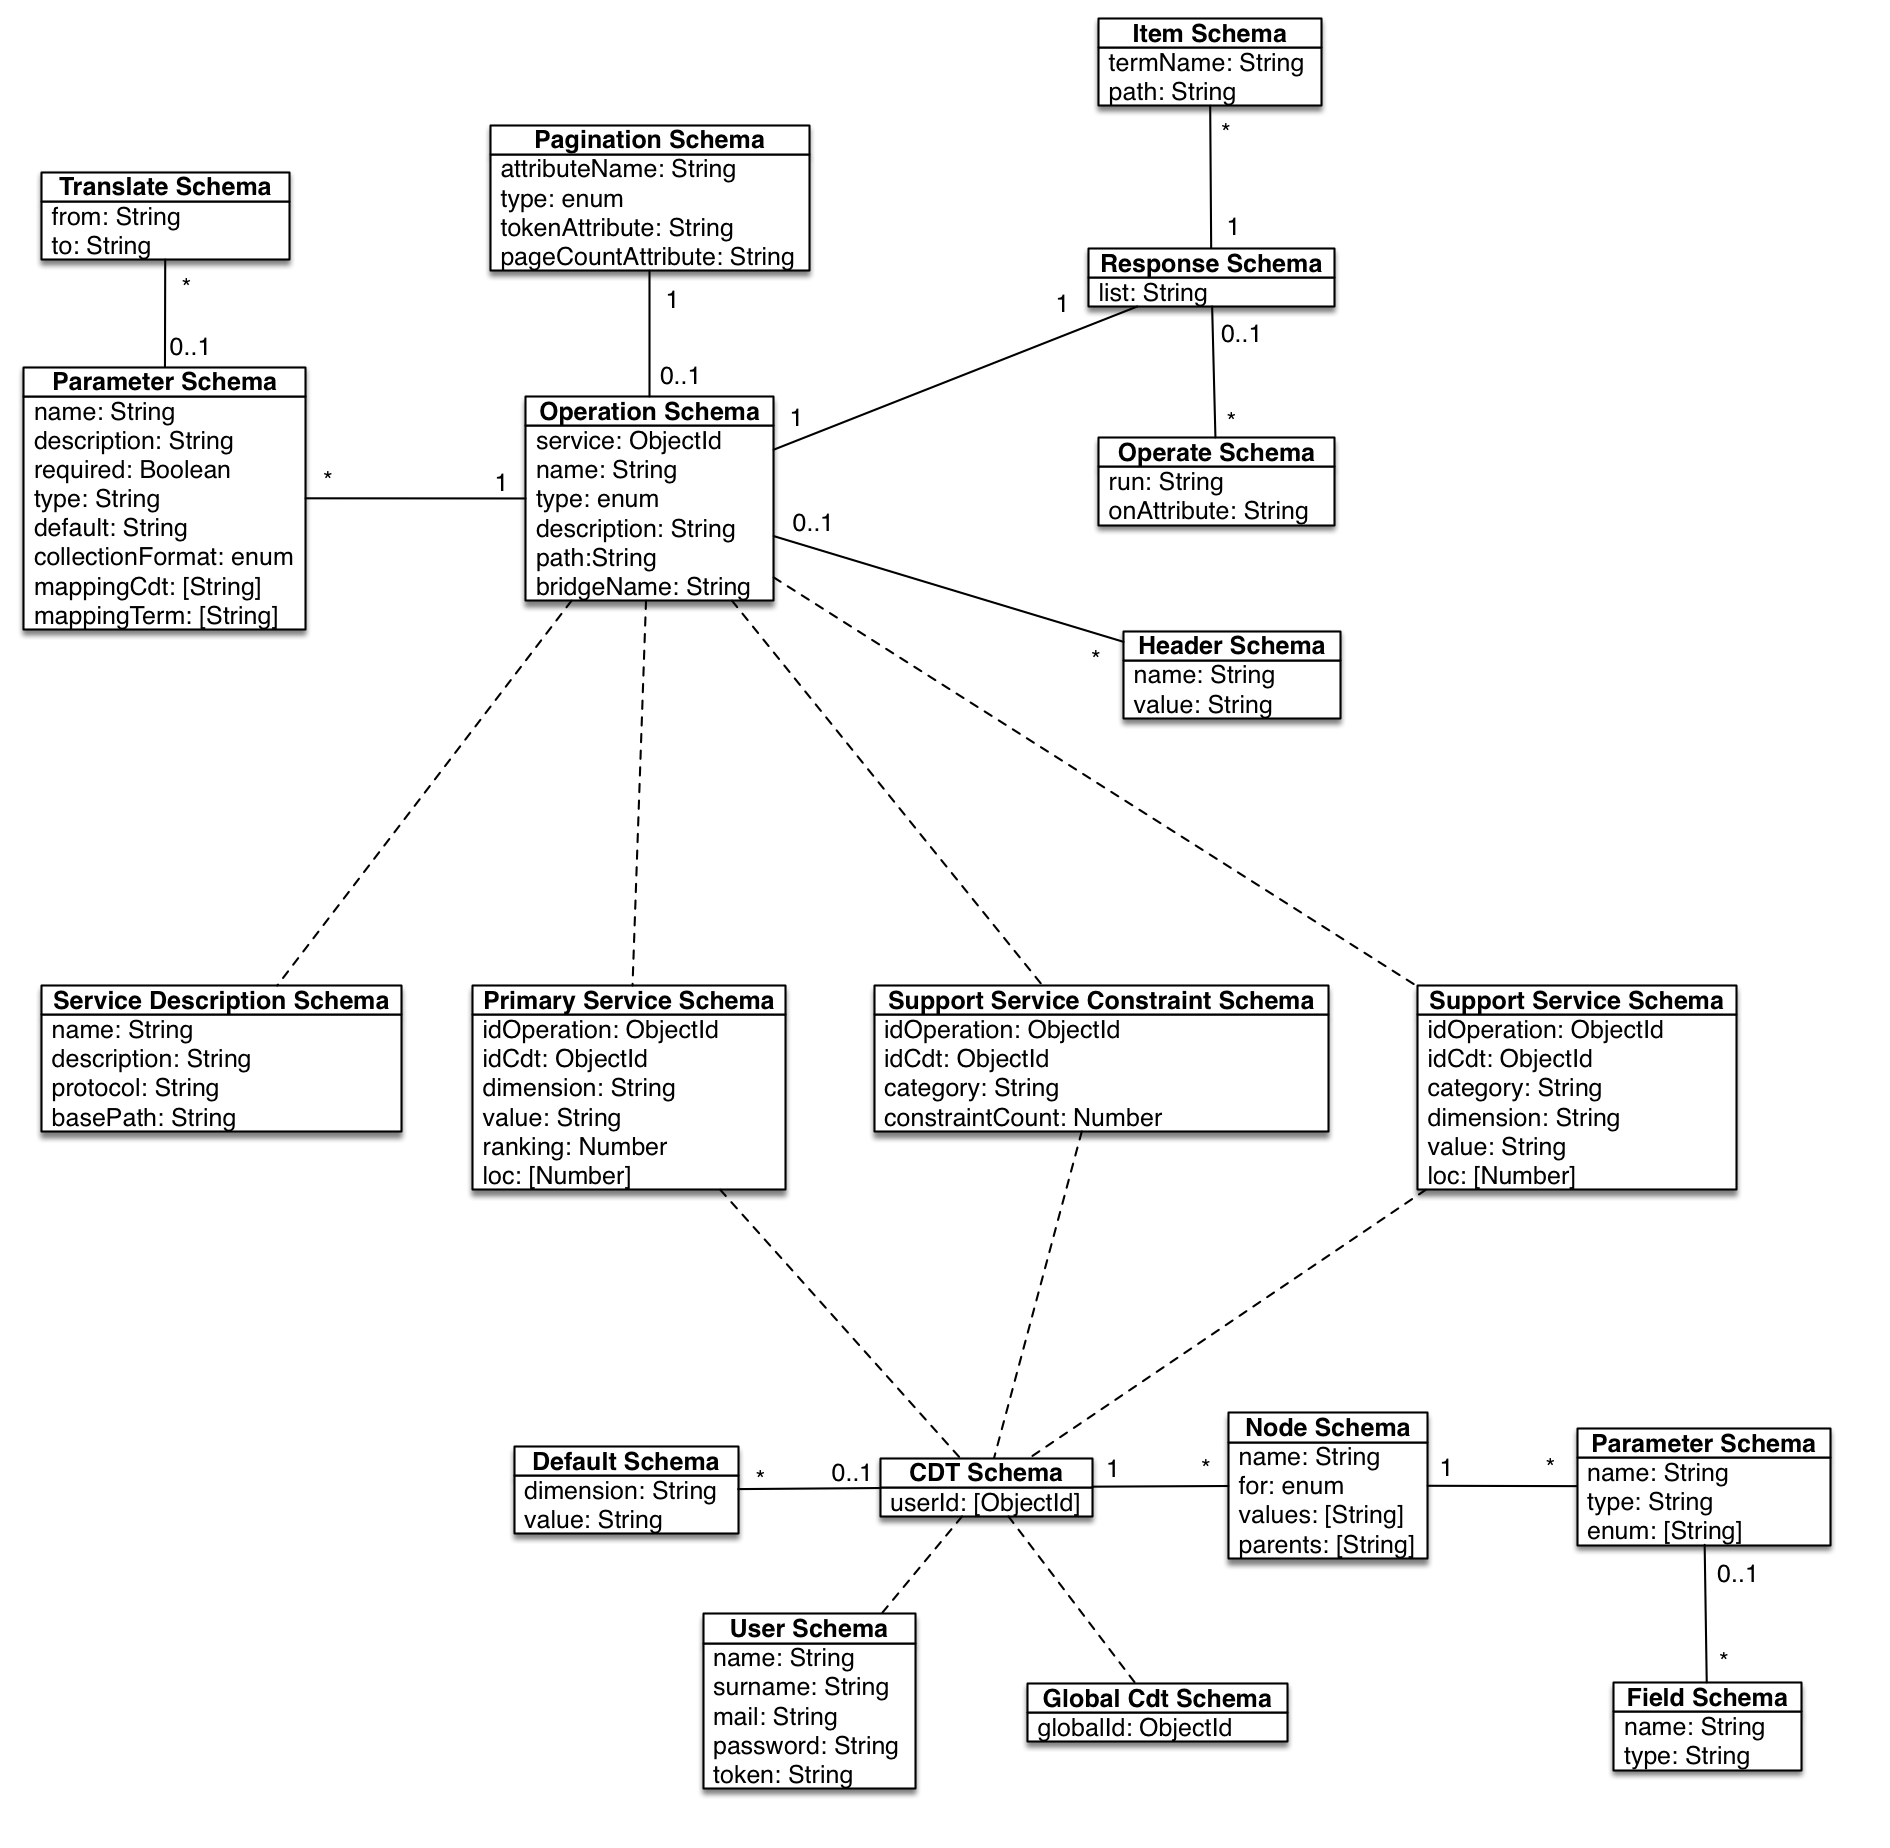
\includegraphics[width=\textwidth]{5-implementazione-backend/Immagini/schema_logico_db.png}
	\caption{Schema logico del database}\label{fig:schema-logico-db}
\end{figure}

\section{Componenti\label{sec:componenti-backend}}

Come già evidenziato nella Sezione \ref{sec:architettura-backend}, l'architettura del backend è composta da diversi \emph{componenti}. Questa soluzione è stata adottata per via dell'elevata flessibilità che garantisce. Ogni componente è specializzato in un compito preciso e il concatenamento di più componenti permette di realizzare funzionalità più complesse per produrre il risultato desiderato. Per svolgere le principali attività vengono dunque create delle \emph{pipeline}, dove il risultato di un componente viene acquisito ed ulteriormente elaborato dal successivo.

Altra caratteristica importante è l'assenza di informazioni sullo stato in ogni componente. Una richiesta nasce nel momento in cui l'utente conferma l'attività e muore una volta che viene evasa. La ragione principale di questa scelta risiede nel fatto che sarebbe oneroso lato backend gestire tutte le informazioni della moltitudine di utenti che sono connessi al sistema. Inoltre mantenere uno stato limiterebbe la scalabilità del sistema, in quanto se un utente inizia la sessione su di un determinato server dovrà continuare sempre su quello, rendendo complicato il bilanciamento dei carichi tra le diverse macchine.

A questo punto è necessaria una importante precisazione: per la gestione della paginazione è necessario l'utilizzo di alcune informazioni sullo stato. Questa affermazione può sembrare un controsenso rispetto a ciò che è stato esposto nel paragrafo precedente. \upe dunque essenziale definire in modo dettagliato cosa si intende per \emph{stato}. La principale differenza consiste nel \emph{dove} vengono salvate le informazioni. Nel paragrafo precedente, ogni volta che si menzionava il concetto di \emph{stato}, si intendeva tutte le informazioni relative l'utente salvate all'\emph{interno} dei componenti, sotto forma di variabile. Questa soluzione, come già affermato anche in precedenza, risulta in un collo di bottiglia non indifferente, in quanto tutte le richieste che nascono in una determinata macchina dovranno essere gestite unicamente da essa. Si è adottata quindi una soluzione differente: i \emph{componenti} non mantengono al loro interno alcuna informazione riguardo lo stato, che verrà memorizzato e reso disponibile da un servizio esterno. Questa soluzione permette a tutti i componenti che ne hanno esigenza di andare a recuperare le informazioni sullo stato da una sorgente comune, che non limita la scalabilità del sistema. Questo servizio può a sua volta offrire dei sistemi di \emph{clustering} per aumentare le perfomance in situazioni di elevato carico.

In CAMUS questa attività viene svolta da Redis, che è stato selezionato per l'elevata rapidità nell'evadere le richieste e nella possibilità di associare un periodo di vita alle informazioni che vengono memorizzate. Viene ipotizzato che dopo un determinato lasso di tempo se l'utente non effettua più interazione sulla sessione, essa può ritenersi estinta e i suoi dati eliminati.

In Figura \ref{fig:class-diagram-backend} viene mostrato il diagramma delle classi di tutti i componenti che formano il backend del sistema.

\begin{figure}[ht]
	\hspace*{-2.2cm}
	\centering
	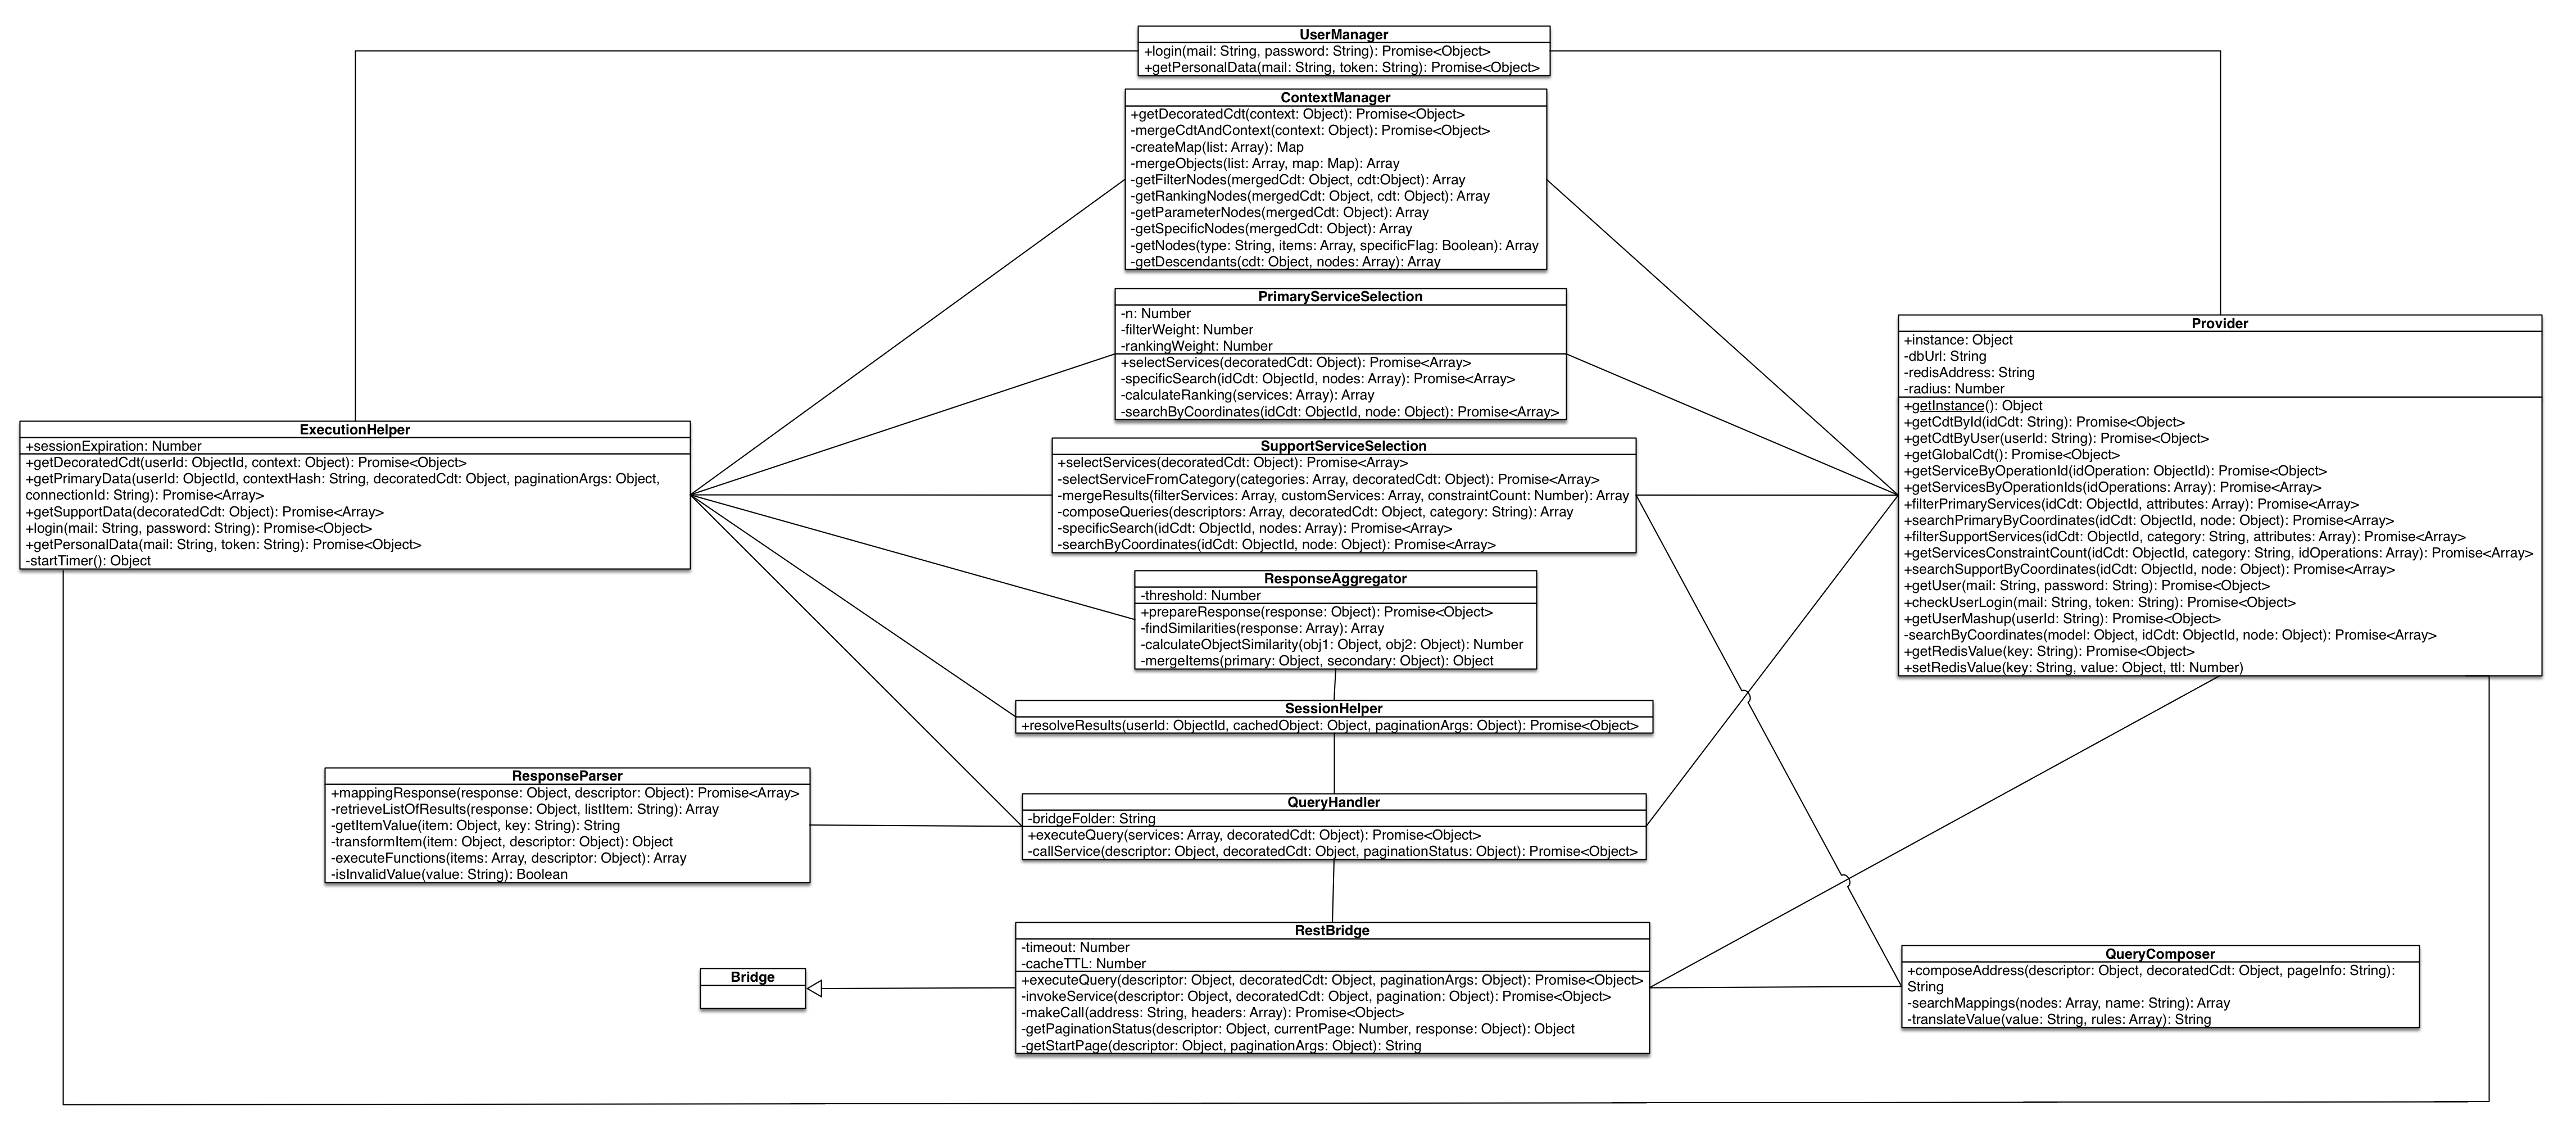
\includegraphics[width=1.4\textwidth]{5-implementazione-backend/Immagini/diagramma_classi_backend.png}
	\caption{Diagramma delle classi del backend}\label{fig:class-diagram-backend}
\end{figure}

Nelle seguenti sottosezioni verranno analizzate nel dettaglio le attività svolte dai componenti principali del sistema.

\subsection{Provider\label{sec:provider}}

Il \emph{Provider} rappresenta il punto di accesso ai database. \upe realizzato seguendo il pattern \emph{singleton}, che prevede una singola istanza della classe in comune per tutti i componenti. Le varie classi che necessitano di accedere al database possono recuperare l'istanza corrente tramite il metodo statico \emph{getInstance()}. Durante l'inizializzazione si occupa di creare le connessioni verso MongoDB e Redis. Implementa tutti i metodi necessari per recuperare le informazioni dal database e centralizza le query tutte in un singolo punto, in modo che gli altri componenti del sistema non debbano preoccuparsi di comporre le clausole. Inoltre, visto che diversi metodi vengono utilizzati da più componenti, si evitano duplicazioni di codice che provocano una riduzione della manutenibilità del sistema, in quanto una modifica ad un metodo dovrebbe essere ripetuta più volte.

I metodi sono stati raggruppati in sei categorie, in base alla funzionalità:

\begin{enumerate}
	\item \textbf{CDT Methods} Mette a disposizione le funzioni necessarie a recuperare gli alberi di contesto
	\item \textbf{Service Descriptor Methods} Definisce le funzioni che vengono utilizzate per acquisire i descrittori dei servizi
	\item \textbf{Primary Service Methods} Fornisce le funzioni di ricerca delle associazioni tra i nodi del CDT e le operazioni primarie
	\item \textbf{Support Service Methods} Implementa i metodi di ricerca delle associazioni tra i nodi del CDT e le operazioni di supporto
	\item \textbf{User Methods} Definisce i metodi che vengono utilizzati per l'autenticazione degli utenti e il recupero delle informazioni personali, quali il proprio \emph{albero di contesto} o i \emph{mashup}
	\item \textbf{Redis Methods} Vengono messi a disposizione i metodi per richiedere o salvare un oggetto in Redis in base alla chiave che si desidera utilizzare
\end{enumerate}

\subsection{Context Manager\label{sec:context-manager}}

Il \emph{Context Manager} è il componente dedicato alla gestione del contesto. Riceve come input il contesto dell'utente, composto dalle coppie $ {<}dimensione, valore{>} $ relative il proprio albero di contesto. La prima attività svolta è quella di \emph{unire} il contesto dell'utente e la descrizione del CDT presente nel database. Per unione si intende associare alla rispettiva dimensione il relativo valore ricevuto.

In seguito inizia la fase di creazione del \emph{CDT decorato}. Questa rappresentazione sarà quella che verrà utilizzata da tutti i componenti che seguono il \emph{Context Manager} nella pipeline. Il \emph{CDT decorato} non è altro che il descrittore del CDT in una forma più comoda per essere utilizzata nelle elaborazioni, in quanto cataloga i nodi dell'albero in quattro categorie ben specifiche, che potranno essere semplicemente recuperate dai componenti che ne hanno bisogno senza la necessità di andare ogni volta a leggere l'intero contesto. In particolare, il CDT decorato è composto dalle seguenti categorie:

\begin{itemize}
	\item \textbf{Filter Nodes} Sono i nodi di tipo filtro che vengono utilizzati per selezionare le operazioni
	\item \textbf{Ranking Nodes} L'elenco dei nodi di tipo ranking che vengono utilizzati per selezionare le operazioni
	\item \textbf{Specific Nodes} Sono i nodi che non utilizzano la ricerca standard delle associazioni ma richiedono una ricerca specifica
	\item \textbf{Parameter Nodes} L'elenco dei nodi dai quali recuperare i valori da utilizzare per la composizione delle query
\end{itemize}

\upe da tenere in considerazione, come precedentemente fatto notare nella Sezione \ref{sec:descrittore-albero-contesto}, che alcuni nodi possono appartenere a più categorie nello stesso tempo. Questa eventualità capita spesso per i nodi che vengono utilizzati sia per filtrare i servizi sia come parametro nella fase di composizione delle query.

Un'altra attività svolta durante la composizione del \emph{CDT decorato} è la ricerca dei nodi figlio. Come definito nella Sezione \ref{sec:associazione-servizi-cdt} le associazioni possono essere specificate sia nei nodi foglia sia in quelli intermedi. \upe importante quindi verificare se un nodo attivo possieda dei figli perché in tal caso anch'essi possono dare un contributo nelle successive fasi di selezione.

\begin{algorithm}
	\caption{Algoritmo di ricerca dei nodi figlio}
	\label{alg:algoritmo-ricerca-nodi-figlio}
	\begin{algorithmic}
		\Require
			\Statex $cdt$ \Comment The decorated CDT
			\Statex $nodes$ \Comment The list of active nodes
		\Ensure
			\Statex $childList$ \Comment List of child nodes found
		\Statex
		\State $nodeValues \gets nodes.map('value')$ \Comment Acquire list of values selected
		\ForAll {$ item\; in\; cdt.context $}
			\State $ intersection \gets intersect(item.parents, nodeValues) $
			\If {$ !isEmpty(interesection) $}
				\ForAll {$ value\; in\; item.values $}
					\State $ childList.push(\{ $
					\State\hspace{\algorithmicindent} $ name: item.name, $
					\State\hspace{\algorithmicindent} $ value: value $
					\State $ \}) $
				\EndFor
			\EndIf
		\EndFor\\
		\Return $ childList $
	\end{algorithmic}
\end{algorithm}

\subsection{Primary Service Selection\label{sec:primary-service-selection}}

Il \emph{Primary Service Selection} è il componente dedicato alla ricerca delle operazioni da interrogare. Riceve come input il \emph{CDT Decorato} e produce in uscita l'elenco degli \emph{identificativi delle operazioni} selezionate, assieme al relativo \emph{punteggio}.

La prima attività svolta riguarda l'acquisizione delle operazioni che sono associate al contesto corrente. Questa fase viene divisa in due fasi:

\begin{enumerate}
	\item \textbf{Ricerca Standard} Viene effettuata cercando nel database tutte le operazioni che sono associate alle coppie $ {<}dimensione, valore{>} $ attive
	\item \textbf{Ricerca Specifica} Utilizza dei metodi specifici per ricercare le associazioni. Un esempio è la ricerca delle operazioni tramite \emph{coordinate}, che sfrutta le funzionalità di MongoDB di effettuare query geospaziali
\end{enumerate}

I risultati della \emph{ricerca standard} vengono a loro volta divisi in base alla tipologia di nodo alla quale sono associati. Le due categorie sono \emph{filter} e \emph{ranking}, alle quali viene assegnato un peso diverso come descritto nella Sezione \ref{sec:selezione-operazioni}. Invece i risultati delle ricerche specifiche vengono classificati sempre come \emph{ranking}.

Una volta acquisite le associazioni attive, viene calcolato il \emph{punteggio} di ogni operazione. Viene utilizzata la Formula \ref{eq:primary-service-formula} per il calcolo del \emph{punteggio} totale di ogni operazione.

Completata questa fase, l'elenco delle operazioni viene riordinato in modo decrescente in base al \emph{punteggio} calcolato e vengono selezionate solamente le Top-N operazioni col punteggio più elevato. 

\subsection{Query Handler\label{sec:query-handler}}

Il \emph{Query Handler} è il componente che orchestra le chiamate verso i servizi primari, riceve le risposte e le trasforma nel formato interno. Riceve come input gli identificativi dei servizi e ne acquisisce i descrittori completi dal database.

Una volta disponibili può iniziare la fase di richiesta delle informazioni. Per svolgere questo compito vengono utilizzati diversi \emph{bridge}. \upe possibile così separare l'implementazione specifica del servizio in un altro componente, in modo che più servizi che condividono la medesima logica possano utilizzare lo stesso bridge. Il \emph{Query Handler} seleziona dunque il bridge idoneo per interrogare il servizio e ne esegue il metodo \emph{executeQuery()}, che si occupa di interrogare il servizio e restituire la risposta. Oltre all'elenco dei risultati, viene restituito un oggetto contenente le informazioni sullo stato della paginazione (es.: se sono disponibili ulteriori pagine o il valore per richiamare la pagina successiva), se il servizio ha una descrizione di come gestire la paginazione.

Quando viene restituita una risposta provvede a \emph{trasformarla} nel formato interno, basandosi sull'utilizzo dei termini semantici da associare agli attributi che compongono la risposta.

Una volta che tutti i servizi hanno risposto e i risultati sono stati trasformati, li integra assieme, accodandoli in un unico vettore, e li restituisce in uscita, pronti per essere ulteriormente elaborati dal componente successivo.

\subsection{Bridge\label{sec:bridge}}

Un \emph{Bridge} è il componente che si occupa di gestire le chiamate verso i servizi esterni e ricevere le risposte. \upe costituito da una classe astratta che deve essere estesa dalle implementazioni specifiche. In questo modo viene lasciata flessibilità di estensione ogni qual volta sia necessaria una logica diversa per invocare un servizio. In particolare viene forzata l'implementazione del metodo \emph{executeQuery()}, che riceve in ingresso il \emph{CDT Decorato} per recuperare i valori definiti dall'utente.

Nella sottosezione seguente viene analizzata l'unica implementazione specifica che viene fornita in dotazione col sistema, quella per l'utilizzo dei servizi di tipo REST.

\subsubsection*{REST Bridge}

Il \emph{REST Bridge} fornisce la logica per interrogare i servizi di tipo REST. La prima attività che svolge è la composizione dell'indirizzo verso il quale il servizio può essere interrogato. Viene utilizzato a tal scopo il \emph{descrittore del servizio}, che definisce i campi necessari per comporre l'indirizzo e dove andare a recuperare i valori da utilizzare. In questa fase entra in gioco anche l'informazione sulla prima pagina da interrogare, nel caso quella corrente non sia la prima chiamata che viene effettuata verso il servizio.

Una volta composto l'indirizzo completo, viene effettuata la chiamata verso il servizio. Le risposte ricevute vengono salvate in cache, quindi questa attività ha due varianti: se il dato è presente in cache, questo viene recuperato e fornito in uscita, altrimenti viene interrogato il servizio ed il risultato fornito viene salvato in cache per utilizzi futuri.

Se il servizio prevede l'utilizzo della paginazione viene analizzata la risposta alla ricerca di informazioni sulla presenza di ulteriori pagine da richiedere. In particolare vengono cercati gli attributi relativi al numero totale di pagine o al token per richiamare la pagina successiva, in base alla tipologia implementata dal servizio.

Infine vengono restituite in uscita la risposta del servizio insieme alle eventuali informazioni riguardo la paginazione, che in particolare sono due: \emph{i)} hasNextPage, che indica se è presente un'altra pagina; \emph{ii)} nextPage, che specifica il numero di pagina o token da utilizzare per richiamare la nuova pagina.

\subsection{Response Aggregator\label{sec:response-aggregator}}

Il \emph{Response Aggregator} entra in gioco una volta che sono stati interrogati tutti i servizi. Riceve in input l'elenco dei risultati già trasformati. Il suo compito è di effettuare diverse attività per pulire i dati o aggiungere ulteriori informazioni. Attualmente nel prototipo viene eseguita unicamente la \emph{ricerca dei duplicati}. Questa attività scorre l'intera lista dei risultati e cerca gli oggetti che sono simili tra loro, cioè che rappresentano la medesima entità reale. Ogni qualvolta che due o più oggetti vengono identificati come duplicati, viene avviata un'attività per unirli in un unico oggetto. Questo oggetto conterrà l'unione delle informazioni che ognuno degli elementi mette a disposizione. In questo modo è possibile creare un entità più ricca rispetto a quelle originali. Nel caso in cui ci sia sovrapposizione, ossia quando due o più entità forniscono lo stesso attributo, viene mantenuto il valore restituito dal servizio col punteggio più alto, che si ipotizza sia quello che mette a disposizione i migliori dati per la situazione corrente. Per un'analisi più approfondita dell'algoritmo di ricerca dei duplicati si fa riferimento all'Algoritmo \ref{alg:algoritmo-rimozione-duplicati}.

Un'ulteriore attività, che non è ancora stata implementata, riguarda l'assegnamento di un \emph{punteggio} ad ogni elemento, in base alle informazioni di contesto disponibili. Per esempio, sarà possibile assegnare un punteggio più alto all'elemento che si trova più vicino rispetto all'utente e, per gli altri elementi, verrà assegnato un punteggio via via decrescente man mano che ci si allontana dal punto di riferimento. Si stanno prendendo in considerazione anche logiche di \emph{selezione fuzzy} per permettere una flessibilità maggiore nell'assegnare i vari punteggi.

Una volta terminate le attività sui dati, viene restituita la nuova lista dei risultati.

\subsection{Support Service Selection\label{sec:support-service-selection}}

Il \emph{Support Service Selection} è il componente dedicato alla selezione delle operazioni di supporto o intent. Riceve in ingresso il \emph{CDT Decorato} che, oltre a contenere le selezioni fatte dall'utente, elenca anche le categorie di servizi che si desidera ricevere. Le categorie servono per raggruppare assieme più servizi che svolgono una funzione simile. In base alle associazioni definite verrà poi selezionato il servizio più idoneo per la situazione corrente. L'attività di selezione che viene descritta viene ripetuta integralmente per ognuna delle categorie, in quanto si vuole ottenere almeno un riscontro per tutte le categorie elencate. Come nel caso delle operazioni primarie, si inizia con la ricerca delle operazioni associate ai nodi attivi del CDT. In questo caso non viene più fatta la divisione tra nodi di tipo \emph{filter} e nodi di tipo \emph{ranking} bensì vengono unite queste due categorie. Invece viene mantenuta la logica di ricerca delle associazioni che richiedono dei metodi specifici. Come già descritto nella Sezione \ref{sec:selezione-operazioni}, per le operazioni di supporto le associazioni vengono intese più come \emph{vincoli}. A questo scopo vengono contestualmente recuperati il numero di vincoli associati alle operazioni per le quali è stata trovata almeno un'associazione. Questo passaggio è essenziale, in quanto si vogliono effettivamente selezionare solamente le operazioni che hanno un numero di vincoli uguale o maggiore di quello preimpostato. Il caso in cui i conteggi siano pari è intuitivo, mentre richiede una spiegazione il fatto che esistano situazioni nelle quali il conteggio sia maggiore rispetto al numero di vincoli. Si prenda come esempio un servizio dei trasporti che espone una operazione. Questa operazione necessita di un parametro che specifica se si preferisce spostarsi col \emph{bus} o con la \emph{metro}. Questo valore viene dunque recuperato dall'albero di contesto, in base alla selezione effettuata dall'utente. Visto che si tratta di una sola operazione, ma è valida per più situazioni, verrà associata a due diversi nodi dell'albero. Il conteggio dei vincoli dovrà invece rimanere pari a uno, come se si fosse effettuata una singola associazione. Infatti non è possibile inserire come valore due, perché altrimenti l'operazione non verrebbe mai selezionata, in quanto risulterebbe sempre una sola associazione.

Una volta che sono state selezionate le operazioni che rispettano il numero di vincoli associato, vengono mantenute solamente le operazioni che hanno il numero massimo di vincoli. La ragione di questa scelta è dovuta al fatto che più vincoli sono rispettati significa che l'operazione è più attinente al contesto.

L'ultimo passaggio riguarda la composizione degli indirizzi delle operazioni selezionate. In seguito l'elenco creato viene restituito in uscita, in modo che sia utilizzabile dalla mobile app.

\subsection{Session Helper\label{sec:session-helper}}

Il \emph{Sessione Helper} viene utilizzato quando è stata effettuata una prima richiesta ai servizi e l'app mobile richiede ulteriori dati. Si occupa di gestire il salvataggio in cache della sessione ed eventualmente, quando il primo result set sta per terminare, richiama un'altra volta i servizi richiedendo la pagina successiva.

Per gestire la paginazione tra backend e app mobile vengono utilizzati due parametri:

\begin{itemize}
	\item \textbf{First} Questo campo specifica il numero di elementi che vengono richiesti
	\item \textbf{After} Definisce il \emph{cursore} di partenza. Verranno quindi restituiti il numero di elementi specificati nell'attributo \virgolette{first} dopo l'elemento con quello specifico identificatore
\end{itemize}

La prima attività che viene eseguita è tenere traccia di quanti elementi sono stati visualizzati dall'utente. Questa informazione è necessaria per conoscere quanti elementi rimangono ancora da visualizzare. A questo punto viene controllato se sono disponibili abbastanza informazioni da mostrare, tramite la formula:

\begin{equation}
	elementi\_mostrati \le totale\_elementi - first - 1
\end{equation}

Dove:

\begin{itemize}
	\item \textbf{elementi\_mostrati} indica il numero di elementi che sono già stati mostrati all'utente
	\item \textbf{totale\_elementi} rappresenta il numero totale di elementi presenti in cache
	\item \textbf{first} è lo stesso attributo descritto in precedenza, che indica quanti elementi sono stati richiesti dal client
\end{itemize}

Se l'equazione è rispettata vengono semplicemente restituiti i dati presenti in cache, altrimenti il \emph{Session Helper} si occupa di recuperare dalla cache le informazioni sui servizi prescelti nella richiesta originale e sulle pagine da richiedere ed effettua le richieste ai servizi, sfruttando in particolare il \emph{Query Handler} ed il \emph{Response Aggregator}.

\subsection{Query Composer\label{sec:query-composer}}

Sia nella Sezione \ref{sec:primary-service-selection} che nella \ref{sec:support-service-selection} è stato menzionato il processo di composizione delle query per interrogare i servizi. \upe stato lasciato volutamente generico in quanto è un'attività non svolta dai rispettivi componenti, bensì dal \emph{Query Composer}. Si è scelto di creare un componente ad-hoc in quanto le due attività hanno delle lievi differenze che però non giustificano l'utilizzo di due logiche differenti. Inoltre la composizione degli indirizzi per i servizi di supporto sfrutta alcune regole che sono implementate per i servizi primari. Da qui l'esigenza di avere un unico metodo che si occupa di analizzare il descrittore dei servizi per comprendere come comporre tra loro i parametri e fornire una query completa.

\begin{algorithm}
	\caption{Algoritmo di composizione degli indirizzi}
	\label{alg:algoritmo-composizione-indirizzi}
	\begin{algorithmic}
		\Require
			\Statex $ descriptor $ \Comment The service descriptor
			\Statex $ decoratedCdt $ \Comment The decorated CDT
			\Statex $ pageInfo $ \Comment Information about pagination  (optional)
		\Ensure
			\Statex $ fullAddress $ \Comment The composed service address
		\Statex
		\State $ querySymbols \gets configureQuerySymbols() $
		\State $ baseAddress \gets descriptor.service.basePath + descriptor.path $
		\State $ nodes \gets union(decoratedCdt.filterNodes, decoratedCdt.parameterNodes) $
		\ForAll {$ param\; in\; descriptor.parameters $}
			\If {$ isEmpty(param.mappingCDT)\; \&\&\; isEmpty(p.mappingTerm) $}
				\If {$ isDefined(param.default) $}
					\State $ value \gets  param.default  $
				\Else
					\If {$ param.required $}
						\State $ Error('Mandatory\; parameter') $
					\EndIf
				\EndIf
			\Else
				\State $ separator \gets configureSeparator(descriptor) $
				\If {$ param.mappingCdt $}
					\State $ value \gets findValueInCdt() $
				\Else
					\State $ value \gets acquireTerm() $
				\EndIf
			\EndIf
			\State $ parameters \gets param.name + querySymbols.assign + value  $
		\EndFor
		\If {$ pageInfo $}
			\State $ fullAddress \gets baseAddress + querySymbols.start + parameters +$
			\State\hspace{\algorithmicindent} $ querySymbols.separator + pageInfo $
		\Else
			\State $ fullAddress \gets baseAddress + querySymbols.start + parameters$
		\EndIf\\
		\Return $ fullAddress $
	\end{algorithmic}
\end{algorithm}

Il primo passo riguarda la selezione dei simboli da utilizzare nella query. Verranno utilizzati simboli diversi nel caso il servizio sia di tipo REST o query. Viene subito composto l'indirizzo di base, ossia quello formato dal \emph{basePath} del servizio ed il \emph{path specifico} dell'operazione. Ora incomincia la vera attività, la composizione dei parametri. Questa fase ha il compito di scorrere l'elenco dei parametri definiti nel descrittore del servizio e verificare se è stato definito un valore. Il valore può essere recuperato dall'\emph{albero di contesto} o tramite i \emph{termini semantici}, in questo ordine. Ovviamente non tutti i parametri devono per forza essere compilati. Esistono due casi in base all'attributo \emph{required}:

\begin{enumerate}
	\item \textbf{Parametro obbligatorio} In questo caso deve per forza essere associato un valore. Se non è presente nessuna associazione nè con il CDT nè con i termini semantici verrà utilizzato il valore predefinito. Se non è stato definito nemmeno un valore predefinito verrà lanciata un'eccezione, in quanto il servizio senza un parametro obbligatorio non è utilizzabile
	\item \textbf{Parametro facoltativo} In questo caso viene cercato prima un valore nell'albero di contesto o tra i termini semantici e, se trovata una corrispondenza, il rispettivo valore viene acquisito ed il parametro entrerà a far parte della query
\end{enumerate}

Durante la ricerca dei valori nell'albero di contesto viene anche eseguita la traduzione del valore, se necessario. Se vengono trovate più di una corrispondenza, i valori sono concatenati assieme e divisi tramite il separatore definito nel descrittore. Una volta acquisiti i valori vengono composti assieme, tramite i vari simboli, a formare la seconda parte dell'indirizzo.

Per terminare l'attività vengono messe assieme tutte le parti. All'indirizzo di base viene aggiunta la parte dei parametri appena composta ed anche l'attributo relativo alla paginazione, se richiesto.

\section{Endpoint GraphQL\label{sec:endpoint-graphql}}

Come già definito nella Sezione \ref{sec:architettura-backend}, per realizzare il punto d'accesso al sistema viene utilizzato GraphQL. In questa sezione si andranno ad analizzare le varie funzionalità fruibili dal client. L'indirizzo da contattare rimane sempre lo stesso per tutti i casi, quello che cambia sarà un parametro nella richiesta che permette di identificare quale attività si desidera svolgere. I nomi delle seguenti sottosezioni rappresentano proprio le attività precedentemente citate. Di seguito verranno identificate per semplicità di espressione col nome di endpoint, visto che il fine ultimo è paragonabile a quello degli endpoint nel mondo REST.

\subsection{Execute Query\label{sec:execute-query-endpoint}}

\upe l'endpoint principale, riceve in ingresso il contesto dell'utente e restituisce le informazioni recuperate, divise in \emph{primarie} e di \emph{supporto}. L'oggetto accettato in ingresso è composto dai seguenti campi:

\begin{itemize}
	\item \textbf{User Id} Rappresenta l'identificativo dell'utente che esegue la query
	\item \textbf{Id Cdt} \upe l'identificativo dell'albero di contesto che si desidera utilizzare
	\item \textbf{Context} Contiene le informazioni di contesto, ossia i nodi che sono attivi. Ogni oggetto è composto dai seguenti attributi:
	\begin{itemize}
		\item \textbf{Dimension} Rappresenta il nome del nodo dimensione
		\item \textbf{Value} Contiene il valore selezionato dall'utente per la dimensione
		\item \textbf{Parameters} Elenca i parametri associati alla dimensioni. Ogni parametro è strutturato come di seguito:
		\begin{itemize}
			\item \textbf{Name} Il nome del parametro
			\item \textbf{Value} Il valore definito dall'utente
			\item \textbf{Fields} Contiene l'elenco dei campi associati al parametro. Ogni campo viene descritto dal proprio \virgolette{nome} e dal \virgolette{valore} che assume
		\end{itemize}
	\end{itemize}
	\item \textbf{Support} Contiene l'elenco delle categorie di servizi di supporto che si vogliono ricevere
\end{itemize}

Una volta ricevuto l'oggetto col \emph{contesto}, tramite l'\emph{Execution Helper} viene creato il \emph{CDT Decorato}. Una volta creato, verrà utilizzato come base per l'acquisizione delle informazioni e la composizione dei servizi di supporto. Viene definito il seguente oggetto come risposta:

\begin{itemize}
	\item \textbf{Connection Id} Identificativo univoco della sessione. Viene utilizzato per segnalare a chi effettua la query se la risposta fa parte di una sessione precedente o si tratta di una nuova
	\item \textbf{Primary Connection} Mette a disposizione l'elenco dei risultati. La particolarità è che si tratta di una \emph{connessione}, che è una tipologia specifica di GraphQL che viene utilizzata quando si ha un elenco di elementi da mostrare. La caratteristica principale che mette a disposizione riguarda la paginazione dei dati. Una volta definita la connessione, sempre tramite l'\emph{Execution Helper}, viene avviato il flusso di richiesta delle informazioni. A GraphQL viene restituito un vettore con i risultati. A partire da questo elenco sarà suo compito dividerlo in parti in base alla richiesta ricevuta dal client. In particolare vengono utilizzati due parametri per specificare quali elementi si desiderano ricevere: \emph{i)} first, dove viene specificato il numero di elementi che si desidera ricevere; \emph{ii)} after, che definisce il cursore dell'ultimo elemento ricevuto nella richiesta precedente. Quando viene utilizzato unicamente il campo \virgolette{first}, GraphQL restituisce i primi N risultati. Se viene specificato anche il campo \virgolette{after} vengono mostrati gli N elementi a partire dall'elemento successivo a quello definito dal cursore. Per cursore si intende un identificativo univoco che viene automaticamente calcolato da GraphQL per ogni elemento della risposta. Per permettere al client di conoscere lo stato della paginazione oltre all'elenco dei risultati viene restituito anche un oggetto di stato, contenente principalmente due attributi: \emph{i)} hasNextPage, valore booleano che indica se può essere recuperata un'ulteriore pagina; \emph{ii)} endCursor, che fornisce il cursore dell'ultimo elemento ricevuto nella richiesta corrente. In questo modo viene lasciata libertà al client di gestire il numero di elementi da ricevere. Ogni oggetto che compone la risposta è composto dai \emph{termini semantici} che sono stati definiti nel sistema. Inoltre viene aggiunto un oggetto che indica da quali servizi, che possono essere più di uno nel caso di unione di elementi duplicati, è stato recuperato l'oggetto e il punteggio assegnato al servizio in fase di selezione
	\item \textbf{Support Connection} Fornisce l'elenco dei servizi di supporto che sono stati selezionati. Come il caso dei risultati primari viene utilizzata una \emph{connessione} di GraphQL. Ogni oggetto viene rappresentato dal \emph{nome} del servizio, la \emph{categoria} per la quale è stato selezionato e l'\emph{indirizzo} composto
\end{itemize}

Nel Listato \ref{lst:esempio-richiesta-execute-query} viene mostrato un esempio di richiesta per effettuare la ricerca di dati sia \emph{primari} sia di \emph{supporto}.

\begin{lstlisting}[caption=Esempio richiesta executeQuery,
								label=lst:esempio-richiesta-execute-query]
~query Restaurant~ {
	!executeQuery! (
		@userId@: ~"USER_ID"~,
		@idCdt@: ~"CDT_ID"~,
		@context@: [
			{
				@dimension@: ~"InterestTopic"~,
				@value@: ~"Restaurant"~
			},
			{
				@dimension@: ~"Location"~,
				@parameters@: [
					{
						@name@: ~"CityCoord"~,
						@fields@: [
							{
								@name@: ~"Latitude"~,
								@value@: ~"45.4788807"~
							},
							{
								@name@: ~"Longitude"~,
								@value@: ~"9.2321363"~
							}
						]
					}
				]
			},
			{
				@dimension@: ~"Transport"~,
				@value@: ~"PublicTransport"~
			}
		],
		@support@: [~"Transport"~]
	)
	{
		!primaryResults! (@first@: ~9~) {
			!data! {
				!title!
				!address!
				!latitude!
				!longitude!
				!meta! {
					!name!
					!rank!
				}
			}
		}
		!supportResults! {
			!data! {
				!category!
				!service!
				!url!
			}
		}
	}
}
\end{lstlisting}

\subsection{Login\label{sec:login-endpoint}}

Questo endpoint è dedicato all'autenticazione degli utenti. Riceve in ingresso l'indirizzo \emph{mail} e la \emph{password}, cifrata con algoritmo SHA1\footnote{SHA1: \url{https://en.wikipedia.org/wiki/SHA-1}}, digitati dall'utente. Se i due parametri corrispondono ad un utente vengono restituiti il suo \emph{identificativo}, utile per le query successive, un \emph{token}, utilizzato per mantenere aperta la sessione, ed il \emph{nome} e \emph{cognome} dell'utente, per personalizzare l'app con le informazioni personali.

Nel Listato \ref{lst:esempio-richiesta-login} viene mostrato un esempio di richiesta per effettuare l'autenticazione dell'utente.

\begin{lstlisting}[caption=Esempio richiesta login,
								label=lst:esempio-richiesta-login]
{
	!login! (
		@mail@: ~"MAIL_ADDRESS"~,
		@password@: ~"ENCRYPTED_PASSWORD"~
	)
	{
		!id!
		!name!
		!surname!
		!token!
	}
}
\end{lstlisting}

\subsection{Get Personal Data\label{sec:get-personal-data-endpoint}}

Questo endpoint provvede a fornire all'utente i suoi dati personali, che possono essere gli \emph{alberi di contesto} ed i \emph{mashup} che gli sono stati associati dall'esperto di settore. In questo modo l'app mobile può recuperare le versioni più aggiornate degli schemi relativi all'utente. In ingresso vengono richiesti l'identificativo dell'\emph{utente} e il \emph{token} ricevuto nella fase di autenticazione. Se i due valori corrispondono, vengono restituiti i dati richiesti. Il formato della risposta viene composto come segue:

\begin{itemize}
	\item \textbf{Cdt} Rappresenta la radice dell'albero di contesto. Un CDT viene definito dai seguenti attributi:
	\begin{itemize}
		\item \textbf{Id Cdt} L'identificativo dell'albero di contesto
		\item \textbf{Context} Contiene le informazioni sul contesto, ossia i nodi che compongono l'albero. Ciascun nodo viene definito come segue:
		\begin{itemize}
			\item \textbf{Name} Il nome del nodo dimensione
			\item \textbf{Values} L'elenco dei possibili valori che può assumere il nodo
			\item \textbf{Parameters} Lista dei parametri associati al nodo. Ogni parametro è composto dai seguenti campi:
			\begin{itemize}
				\item \textbf{Name} Il nome dell'attributo
				\item \textbf{Type} La tipologia di dato
				\item \textbf{Fields} Elenco di campi che specializzano il parametro. La struttura di un campo è molto simile a quella del parametro, infatti contiene gli attributi \virgolette{Name}, che definisce il nome del campo, e \virgolette{Type}, che ne specifica la tipologia
			\end{itemize}
			\item \textbf{Parents} Elenco di tutti i parenti del nodo corrente
		\end{itemize}
		\item \textbf{Default Values} Elenco dei valori che non vengono mostrati nell'albero di contesto perché precedentemente selezionati. Questo oggetto è composto dagli attributi \virgolette{dimension}, che rappresenta il nome del nodo dimensione, e \virgolette{value}, che è il valore associato al nodo
	\end{itemize}
	\item \textbf{Mashup} Rappresenta lo schema dei mashup. Fornisce all'app mobile le regole per comporre l'interfaccia grafica nelle diverse situazioni. Uno schema di mashup è composto dai seguenti campi:
	\begin{itemize}
		\item \textbf{List} Questo oggetto fornisce le regole per rappresentare la lista dei risultati, ossia la schermata di \emph{merge} o \emph{master}. In questa pagina viene mostrato l'elenco dei dati recuperati, descritti da un insieme ridotto di attributi. Per specificare quali dati devono essere mostrati e come vengono utilizzati i seguenti attributi:
		\begin{itemize}
			\item \textbf{Topics} Elenco degli \emph{Interest Topic} per i quali lo schema corrente è valido
			\item \textbf{Contents} Definisce i componenti che devono essere utilizzati, il loro stile e dove recuperare i dati da essere mostrati. Ogni oggetto viene definito dai seguenti attributi:
			\begin{itemize}
				\item \textbf{Type} Specifica la tipologia di componente da utilizzare (es.: \emph{text} per informazioni testuali, \emph{map} per mostrare una mappa, \emph{website} per creare un collegamento verso una pagina web, ecc.)
				\item \textbf{Style} Permette di definire uno stile diverso da quello predefinito al componente. Se è presente lo stile originale viene completamente ignorato
				\item \textbf{Contents} Definisce quali sono i \emph{termini semantici} dai quali è possibile recuperare le informazioni. Viene inoltre data la possibilità di inserire dei sottocomponenti, dello stesso tipo definito nell'attributo \virgolette{Type}, per formare un componente aggregato
			\end{itemize}
		\end{itemize}	
		\item \textbf{Details} Questo oggetto definisce la composizione della schermata di dettaglio di un singolo elemento. Questa pagina viene richiamata una volta che l'utente seleziona un elemento per controllarne le informazioni specifiche. Viene definito dagli stessi attributi della sezione \virgolette{List}			
	\end{itemize}
\end{itemize}

Nel Listato \ref{lst:esempio-get-personal-data} viene mostrato un esempio di richiesta per ricevere i dati personali dell'utente.

\begin{lstlisting}[caption=Esempio richiesta getPersonalData,
								label=lst:esempio-get-personal-data]
{
	!getPersonalData! (
		@id@: ~"USER_IDENTIFIER"~,
		@token@: ~"SESSION_TOKEN"~
	)
	{
		!cdt! {
			!idCdt!
			!context! {
				!name!
				!values!
				!parameters! {
					!name!
					!type!
					!fields! {
						!name!
						!type!
					}
				}
				!parents!
			}
			!defaultValues! {
				!dimension!
				!value!
			}
		}
		!mashup! {
			!list! {
				!topics!
				!contents! {
					!type!
					!style!
					!contents!
				}
			}
			!details! {
				!topics!
				!contents! {
					!type!
					!style!
					!contents!
				}
			}
		}
	}
}
\end{lstlisting}

\section{Flusso di una richiesta\label{sec:flusso-richiesta-server}}

In questa sezione viene analizzato il flusso di esecuzione principale del sistema, quello che riguarda le richieste proveniente dalla mobile app. Le prime attività che svolge sono il login dell'utente, tramite l'endpoint \emph{login} (Sezione \ref{sec:login-endpoint}), e l'acquisizione dei dati personali dell'utente, tramite l'endpoint \emph{getPersonalData} (Sezione \ref{sec:get-personal-data-endpoint}).

L'attività più importante riguarda invece l'endpoint \emph{executeQuery} (Sezione \ref{sec:execute-query-endpoint}), che è dedicato all'invio delle informazioni trovate in base al contesto dell'utente. In Figura \ref{fig:flusso-nuova-richiesta} vengono mostrati i componenti coinvolti in questa fase e l'ordine col quale sono eseguiti.

\begin{figure}[ht]
	\centering
	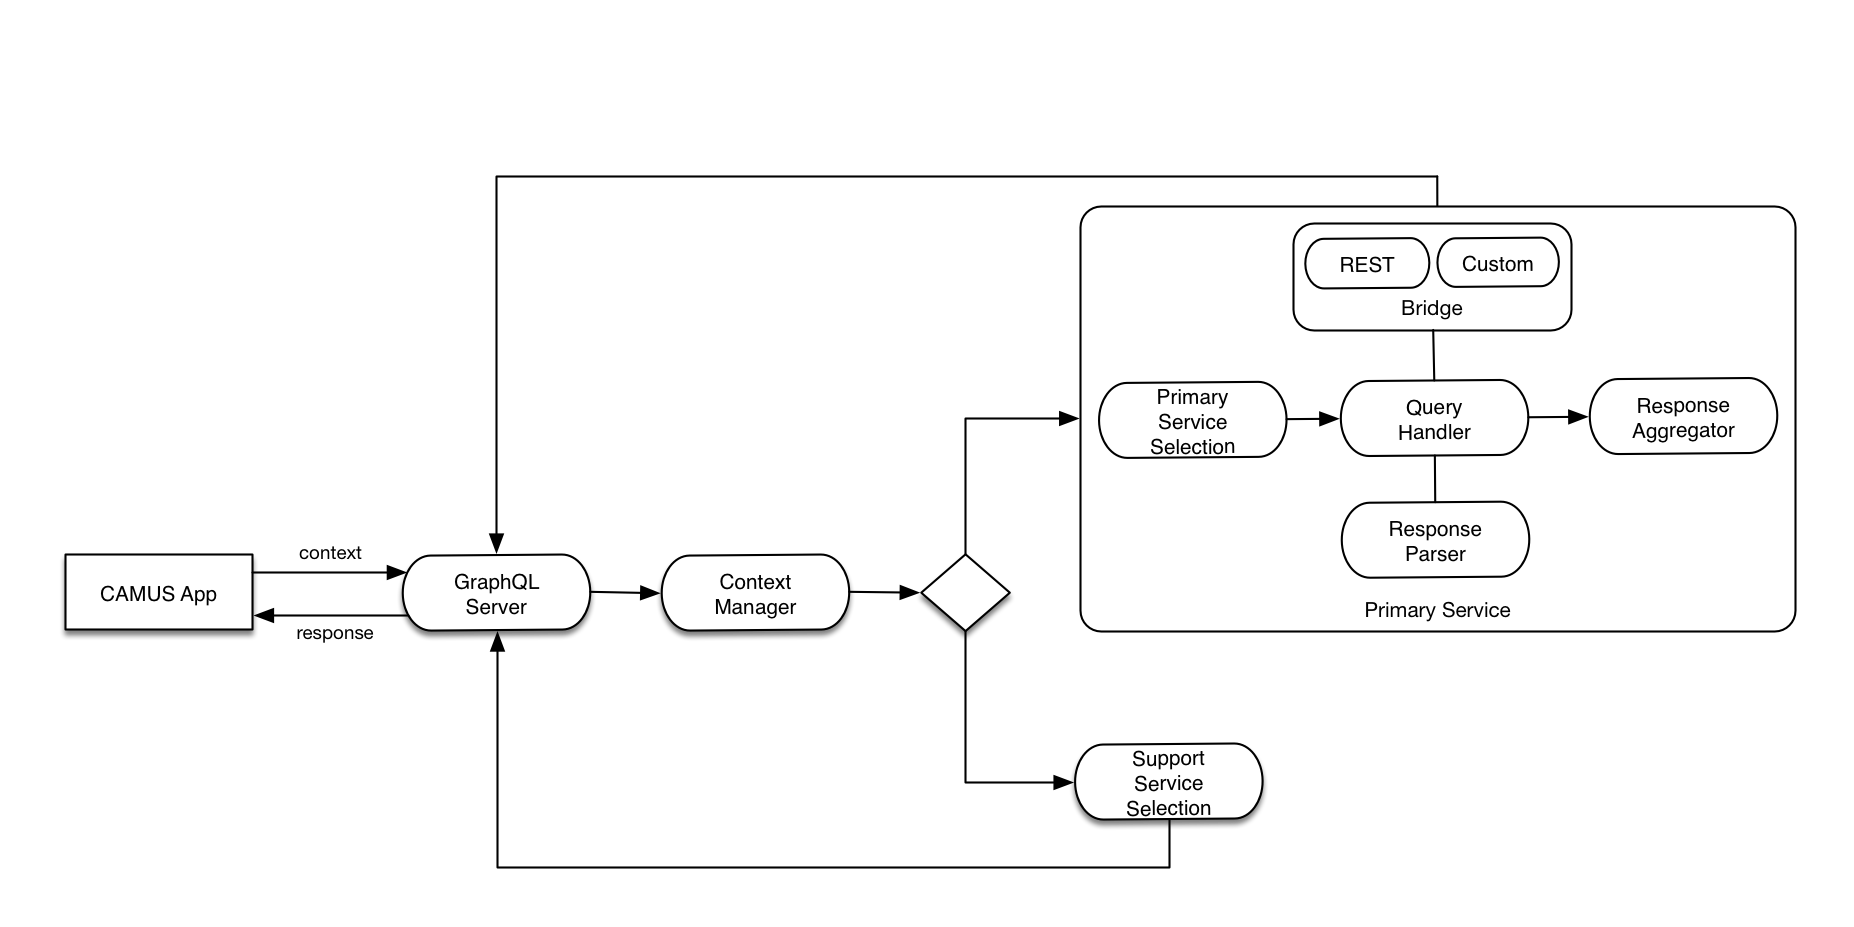
\includegraphics[width=\textwidth]{5-implementazione-backend/Immagini/flusso_richiesta.png}
	\caption{Flusso di una nuova richiesta\label{fig:flusso-nuova-richiesta}}
\end{figure}

L'attività viene divisa in tre fasi:

\begin{enumerate}
	\item \textbf{Creazione CDT decorato} \upe la prima fase che viene eseguita. Una volta ricevuto il \emph{contesto} dal client, questo viene analizzato e trasformato nella versione \emph{decorata}
	\item \textbf{Acquisizione dati primari} Questa fase avviene dopo la creazione del CDT decorato. Si occupa di selezionare le operazioni attinenti al contesto, interrogare i servizi, integrare le risposte ed inviare i dati finali al client
	\item \textbf{Composizione servizi di supporto} Questa fase avviene dopo la creazione del CDT ed in parallelo all'acquisizione dei dati primari. A partire dal contesto si occupa di selezionare i servizi di supporto richiesti dal client e ne compone le query
\end{enumerate}

Nelle successive sottosezioni verranno analizzate nel dettaglio ognuna delle precedenti fasi.

\subsection*{Creazione del CDT decorato}

\upe la prima attività che viene eseguita, della quale si occupa il \emph{Context Manager}. In Figura \ref{fig:flusso-decorated-cdt} viene mostrato il diagramma di flusso delle attività svolte. Riceve in ingresso il \emph{contesto} che è stato composto dall'utente e lo trasforma nella relativa versione \emph{decorata}. Se il contesto è già stato ricevuto in una precedente richiesta, viene recuperata dalla cache la versione decorata che è già stata elaborata, altrimenti viene avviato il processo di trasformazione. Al fine di identificare univocamente ogni contesto, per poterlo memorizzare e recuperare in cache, viene generato un \emph{hash} sull'oggetto ricevuto. In questo modo è possibile anche condividere un contesto tra più utenti diversi.

\begin{figure}[ht]
	\centering
	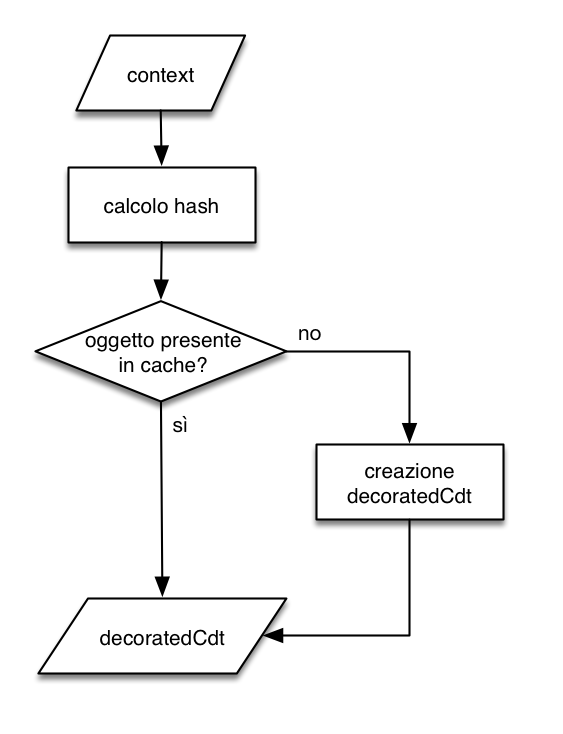
\includegraphics[width=0.43\textwidth]{5-implementazione-backend/Immagini/diagramma_flusso_decoratedCdt.png}
	\caption{Flusso di creazione del CDT decorato\label{fig:flusso-decorated-cdt}}
\end{figure}

\subsection*{Acquisizione dei dati primari}

Questa fase viene eseguita una volta terminata la creazione del \emph{CDT decorato}. In Figura \ref{fig:flusso-servizi-primari} viene mostrato il diagramma di flusso che mostra come viene gestita una richiesta.

La prima attività che viene svolta riguarda il controllo, come nel passaggio precedente, se la richiesta era già stata gestita in passato. Se si tratta di una nuova richiesta, l'attività viene svolta dai componenti che fanno parte del blocco \virgolette{Primary Service} nella Figura \ref{fig:flusso-nuova-richiesta}. Il primo componente che viene eseguito è il \emph{Primary Service Selection}, che si occupa di selezionare le operazioni che sono più idonee al contesto fornito dall'utente. Prodotto l'elenco entra in gioco il \emph{Query Handler}, che ha un duplice compito. Il primo, con l'ausilio di uno o più \emph{Bridge}, è l'invocazione dei servizi prescelti e l'acquisizione delle relative risposte. Una volta ricevute le risposte provvede a trasformarle nel formato interno, tramite le funzioni messe a disposizione dal \emph{Response Parser}. Tutte le risposte ricevute vengono infine unite a formare un'unica lista e restituite per essere ulteriormente elaborate dal \emph{Response Aggregator}, che effettua un'attività di rimozione dei duplicati. L'elenco dei risultati identificato verrà dunque salvato per un periodo di tempo in cache in modo da poter essere riutilizzato per richieste future.

La seconda eventualità si verifica quando la risposta è presente in cache. Questo caso ha una gestione un po' più complessa rispetto al precedente perché viene considerata anche la paginazione dei risultati. La prima verifica riguarda la disponibilità di informazioni da restituire al client. Se la quantità di dati contenuti in cache è sufficiente ad evadere la richiesta viene subito restituita la porzione di informazioni richiesta. Altrimenti viene effettuata una nuova richiesta verso i servizi che hanno ulteriori dati da mostrare. La regola di ricaricamento dei dati è la stessa descritta nella Sezione \ref{sec:session-helper}. Qualsiasi casistica termina sempre con l'aggiornamento dello stato nella cache, in quanto vengono sia salvati l'elenco dei risultati sia il numero di elementi che il client ha già richiesto. Il processo termina una volta che tutti i servizi non ha più dati da mostrare. In quel caso il client verrà informato del fatto che non sono più disponibili ulteriori pagine.

\begin{figure}[ht]
	\centering
	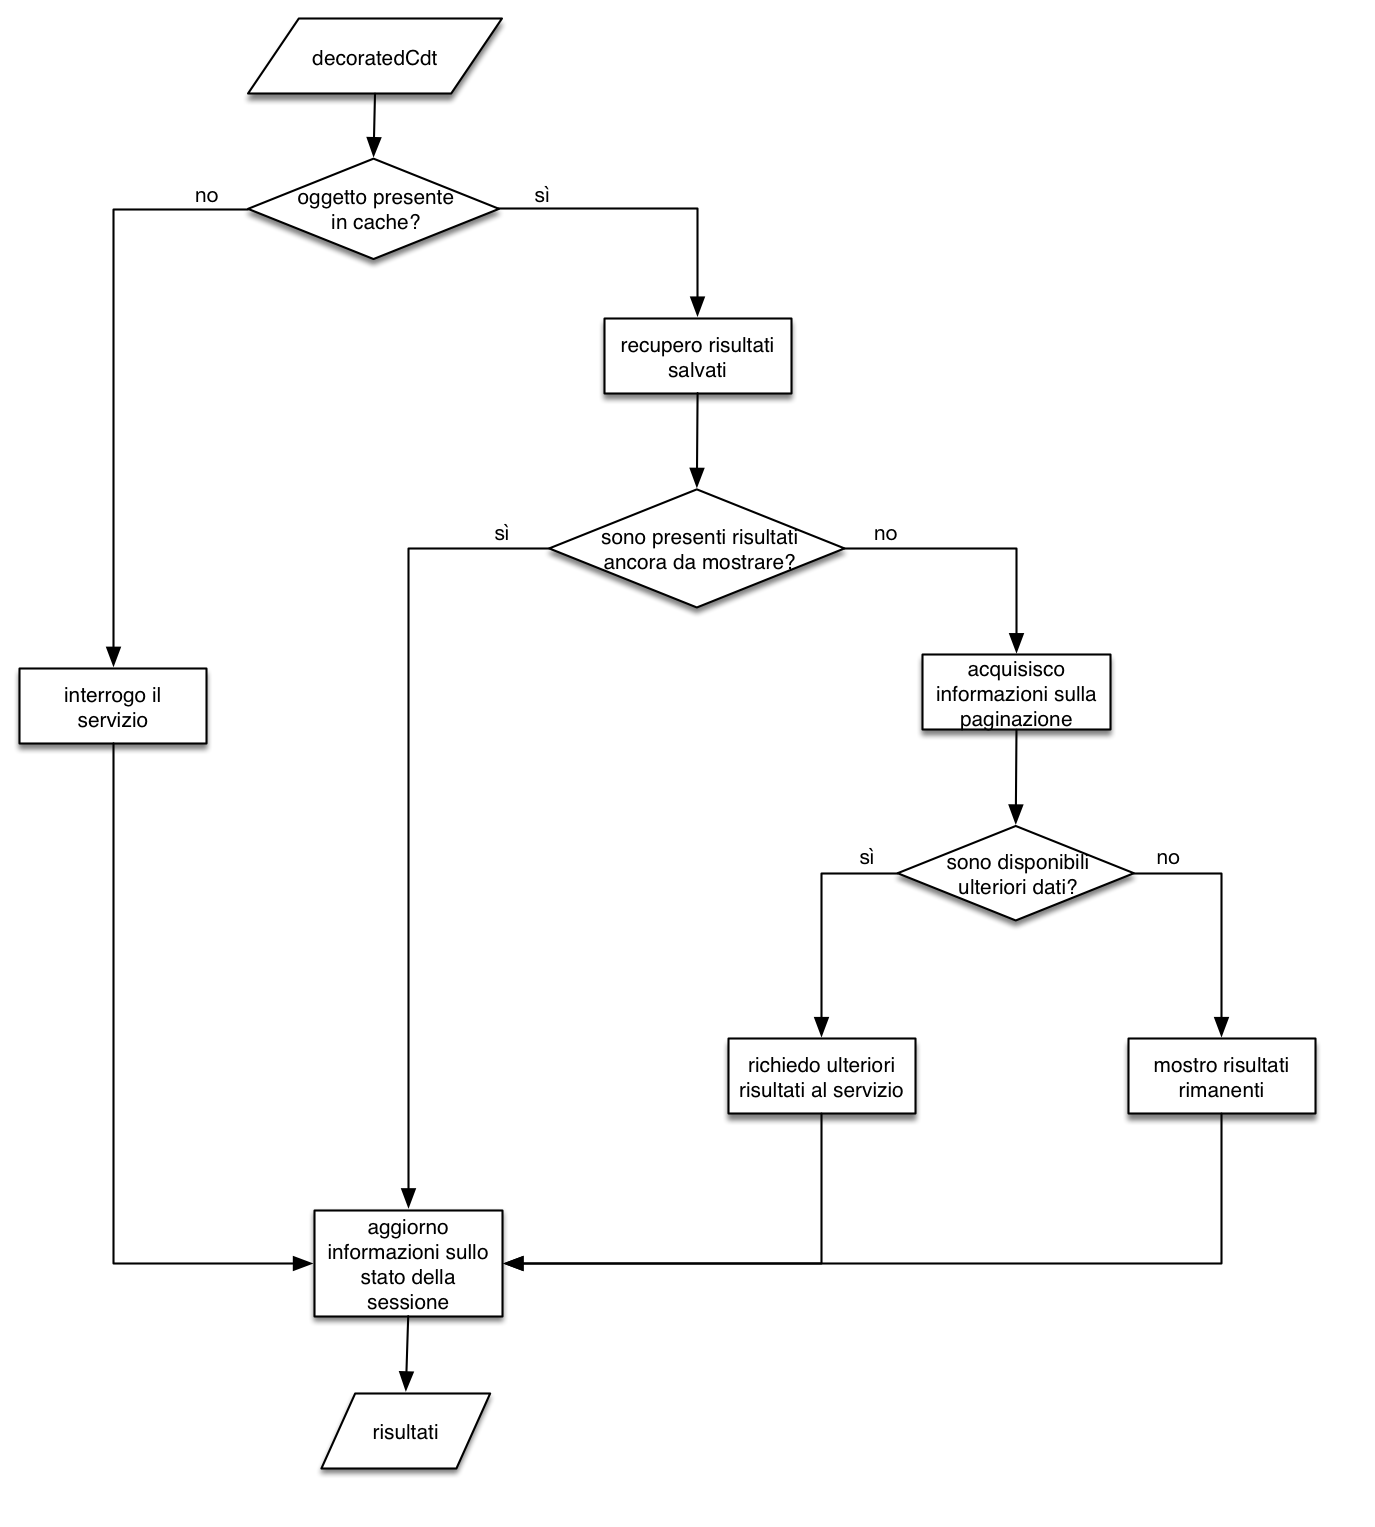
\includegraphics[width=\textwidth]{5-implementazione-backend/Immagini/diagramma_flusso_servizi_primari.png}
	\caption{Flusso di richiesta dei risultati primari\label{fig:flusso-servizi-primari}}
\end{figure}

\subsection*{Acquisizione dei servizi di supporto}

Questa attività incomincia una volta creato il \emph{CDT decorato} ed opera in parallelo all'acquisizione dei servizi primari. Coinvolge unicamente il componente \emph{Support Service Selection}, che si occupa di selezionare i servizi di supporto o gli intent richiesti dal client. In ingresso viene fornita la \emph{categoria} dei servizi che si vuole selezionare in base al contesto fornito.

Una volta selezionati incomincia la fase di composizione delle URL necessarie per interrogare il servizio o richiamare l'intent specifico.

In Figura \ref{fig:flusso-servizi-supporto} viene mostrato il semplice flusso delle attività svolte dal \emph{Support Service Selection}.
	
\begin{figure}[ht]
	\centering
	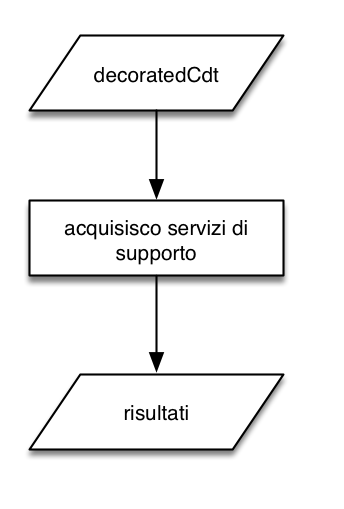
\includegraphics[width=0.3\textwidth]{5-implementazione-backend/Immagini/diagramma_flusso_servizi_supporto.png}
	\caption{Flusso di richiesta dei risultati di supporto\label{fig:flusso-servizi-supporto}}
\end{figure}

\section{File di configurazione\label{sec:file-configurazione}}

Per configurare agilmente determinati parametri del sistema, vengono sfruttate le \emph{variabili d'ambiente} e viene messa a disposizione una cartella dove aggiungere dei \emph{file di configurazione}. In caso di conflitto viene seguita la seguente scala di priorità:

\begin{enumerate}
	\item \textbf{Variabili d'ambiente} Vengono inizialmente considerate le variabili d'ambiente
	\item \textbf{File di configurazione} Il valore viene acquisito dal file di configurazione
	\item \textbf{Valore predefinito} Se nessuno dei due precedenti passi ha prodotto un valore ne viene utilizzato uno predefinito. Esistono casi dove un valore predefinito non è utilizzabile (es.: indirizzo del database), quindi se non viene specificato alcun valore l'applicazione lancerà un'eccezione
\end{enumerate}

Vengono messe a disposizione le seguenti variabili d'ambiente:

\begin{itemize}
	\item \textbf{NODE\_ENV} Per definire l'ambiente nel quale avviare l'applicazione (es.: production, development, testing, ecc.)
	\item \textbf{PORT} La porta che si vuole utilizzare per richiamare gli endpoint
	\item \textbf{MONGOLAB\_URI} L'indirizzo di MongoDB. Può comprendere anche l'utente e la password di accesso al database
	\item \textbf{REDIS\_URL} L'indirizzo di Redis. Può comprendere anche l'utente e la password di accesso al database
\end{itemize}

Nella cartella \virgolette{config} è possibile aggiungere dei file per configurare altri parametri. Possono essere creati più file di configurazione, che verranno caricati per i diversi ambienti nel quale può funzionare l'applicazione. Basta chiamare il file col nome dell'ambiente di destinazione (es.: production, development, qa, staging, ecc.) affinché venga selezionata la configurazione corretta. Viene fornita una configurazione di \virgolette{default}, utilizzata quando non è presente nessun file relativo all'ambiente corrente. Di seguito vengono elencati i parametri che possono essere configurati; tra parentesi sono indicati i valori predefiniti di ciascun campo:

\begin{itemize}
	\item \textbf{server} Contiene la configurazione del server
	\begin{itemize}
		\item \textbf{port} (3001) Definisce la porta che si vuole utilizzare per richiamare l'endpoint
	\end{itemize}
	\item \textbf{database} Contiene la configurazione di MongoDB
	\begin{itemize}
		\item \textbf{address} Definisce l'indirizzo del database. Possono essere incluse le informazioni di autenticazioni
	\end{itemize}
	\item \textbf{redis} Definisce la configurazione di Redis
	\begin{itemize}
		\item \textbf{address} (localhost:6379) Specifica l'indirizzo del database in-memory. Possono essere incluse le informazioni di autenticazioni
	\end{itemize}
	\item \textbf{rest} Specifica la configurazione del bridge per i servizi REST
	\begin{itemize}
		\item \textbf{timeout} Definisce i periodi di tempo dopo i quali scatta il timeout
		\begin{itemize}
			\item \textbf{service} (3000) Valore di timeout dopo il quale una richiesta verso i servizi esterni scade. Il valore viene specificato in millisecondi (ms)
			\item \textbf{cache} (1800) Specifica il tempo per il quale rimangono salvati in cache le risposte ricevute dai servizi. Il tempo viene espresso in secondi (s)
		\end{itemize}
	\end{itemize}
	\item \textbf{primaryService} Gestisce la configurazione del componente \emph{Primary Service Selection}
	\begin{itemize}
		\item \textbf{n} (3) Definisce quante operazioni selezionare
		\item \textbf{weight} Specifica i pesi che vengono assegnati alle varie tipologie di nodo
		\begin{itemize}
			\item \textbf{filter} (1) Peso dei nodi di tipo \emph{filter}
			\item \textbf{ranking} (4) Peso dei nodi di tipo \emph{ranking}
		\end{itemize}
	\end{itemize}
	\item \textbf{similarity} Configurazione del componente di ricerca dei duplicati
	\begin{itemize}
		\item \textbf{threshold} (0.85) Definisce la percentuale minima di similarità tra due elementi affinché vengano considerati duplicati. Una valore maggiore indica un'elevata similarità tra gli elementi. Viene considerato come una percentuale (es.: 0.9 equivale al 90\% di similarità)
	\end{itemize}
	\item \textbf{paginationTTL} (1800) Definisce il tempo per il quale rimane memorizzato lo stato di una connessione in cache. Il tempo viene specificato in secondi (s)
	\item \textbf{debug} (false) Indicatore booleano che abilita o disabilita il logging delle informazioni su console
	\item \textbf{metrics} (false) Valore booleano che abilita o disabilita la raccolta delle informazioni sui tempi di esecuzione dei metodi principali e delle chiamate verso i database
\end{itemize}

Nessun campo è obbligatorio, ad eccezione dell'indirizzo di MongoDB, se non specificato tramite \emph{variabili d'ambiente}. In assenza degli altri campi verranno utilizzati i rispettivi valori di default.

Nel Listato \ref{lst:file-configurazione-predefinito} viene mostrato il file di configurazione predefinito.

\begin{lstlisting}[style=blocco-esempi,
								caption=File di configurazione predefinito,
								label=lst:file-configurazione-predefinito]
{
	"server": {
		"port": 3001
	},
	"database": {
		"address": "mongodb://localhost/camus"
	},
	"redis": {
		"address": "localhost:6379"
	},
	"rest": {
		"timeout": {
			"service": 3000,
			"cache": 1800
		}
	},
	"primaryService": {
		"n": 3,
		"weight": {
			"filter": 1,
			"ranking": 4
		}
	},
	"similarity": {
		"threshold": 0.85
	},
	"paginationTTL": 1800,
	"debug": true,
	"metrics": true
}
\end{lstlisting}